% The font can be either 10pt or 12pt to conform to UNCC standards.  Change it here if you like.
\documentclass[12pt]{article}

%%%%%%%%%%%%%%% The base packages required by the Graduate School. Modify these  at your own peril!%%%%%%%%%%%%%%% 

\usepackage{packages/thesis}
% This line makes sure that single-line captions won't automatically center. 
\usepackage{caption} % Should this move to unccspecs.sty?

%packages Drew added
\usepackage{mathptmx}
\usepackage{graphicx}
\usepackage{subfigure}
\usepackage[bookmarks,backref=true,linkcolor=black]{hyperref} %,colorlinks
\hypersetup{
  pdfauthor = {},
  pdftitle = {},
  pdfsubject = {},
  pdfkeywords = {},
  colorlinks=true,
  linkcolor= black,
  citecolor= black,
  pageanchor=true,
  urlcolor = black,
  plainpages = false,
  linktocpage
}

\captionsetup{singlelinecheck=false}
%%%%%%%%%%%%%%%%%%%%%%%%%%%%%%%%%%%%%%%%%%%%%%%%%%%%%%%%%%%%%%%%%%%%%%%%%%%%%%%


%%%%%%%%%%%%%%% OPTIONAL PACKAGES YOU MAY WANT TO CONSIDER %%%%%%%%%%%%%%%
% Uncomment the \usepackage{} command to add the environments to your document. Note that Miktex may need to download the package the first time you add the package, so be patient, especially if you enable a lot of these packages at once.

% Add colors to your text.  Excellent tool for leaving yourself notes. (http://en.wikibooks.org/wiki/LaTeX/Colors)
%\usepackage{color}

% It supplies a landscape environment, and anything inside is basically rotated. (http://en.wikibooks.org/wiki/LaTeX/Page_Layout)
%\usepackage{lscape}

% A set of useful symbol fonts (http://www.ctan.org/pkg/ifsym)
%\usepackage{ifsym}

% supports the creation of indices, like at the end of most books (http://en.wikibooks.org/wiki/LaTeX/Indexing)
%\usepackage{makeidx}

% Allows the manipulation of graphics (http://en.wikibooks.org/wiki/LaTeX/Importing_Graphics)
%\usepackage{graphicx}

% 	The package alters the command \_ (which normally prints an underscore character or facsimile) so that the hyphenation of constituent words is not affected, and hyphenation is permitted after the underscore. (http://ctan.mirrorcatalogs.com/macros/latex/contrib/underscore/underscore.pdf)
%\usepackage{underscore}

%  Everything input between the begin and end commands are processed as if by a typewriter (http://en.wikibooks.org/wiki/LaTeX/Paragraph_Formatting). Useful for adding code blocks/listings
%\usepackage{verbatim}

%  Used with verbatim to include the source code of any programming language within your document
%\usepackage{listings}

% Helps format tables using the \toprule, \midrule, and \bottomrule commands (http://en.wikibooks.org/wiki/LaTeX/Tables#Using_booktabs)
%\usepackage{booktabs}

%  Helps format tables (http://en.wikibooks.org/wiki/LaTeX/Tables#Using_array)
%\usepackage{array}

% Allows columns spanning multiple rows in the table environment (http://en.wikibooks.org/wiki/LaTeX/Tables)
%\usepackage{multirow}

% Allows rotating of any object (http://en.wikibooks.org/wiki/LaTeX/Rotations)
%\usepackage{rotating}

% Allows captions in figures and tables. Especially useful when used with subcaptions if doing subfigures (http://en.wikibooks.org/wiki/LaTeX/Floats,_Figures_and_Captions)
%\usepackage{caption}

% Will arrange the figures or tables side-by-side (http://en.wikibooks.org/wiki/LaTeX/Floats,_Figures_and_Captions)
%\usepackage{subcaption}

% Balances columns on the last page. Not very useful here, but very useful in scholarly papers to balance your last page (http://www.ctan.org/pkg/flushend)
%\usepackage{flushend}

% Inserts hypertext markups into document (so digital copies have a table of contents which links to chapters, sections, figures, etc.) (https://www.tug.org/applications/hyperref/manual.html)
%\usepackage[pdftex]{hyperref}

% Creates a compact list (http://www.howtotex.com/packages/compact-lists-with-paralist/)
%\usepackage{paralist}
%%%%%%%%%%%%%%%%%%%%%%%%%%%%%%%%%%%%%%%%%%%%%%%%%%%%%%%%%%%%%%%%%%%%%%%%%%%%%%%


% This line decides how deep the Table of Contents will go.  
% A tocdepth of 1 means it will only show chapters and sections.
% You can increase it if you want your Table of Contents to show 
% subsections (tocdepth = 2) or subsubsections (tocdepth = 3) as well.
\setcounter{tocdepth}{2}

\begin{document}

% !!!!!!!!!!!! WARNING !!!!!!!!!!!!!!
%
% When printing your thesis, pay attention to the "Page Scaling" option on the print setup page!
% DO NOT choose the option "Fit to Printable Area."
% This is the default option in Adobe and it will make your formatting wrong!
%  Make sure you change this option to "None."
%
% !!!!!!!!!!!!!!!!!!!!!!!!!!!!!!!!!!!!!!!!

\startprelim

\author{Drew Skau}
\title{Supporting Creativity in the Creation of Data Visualizations Without Programming Using An Object-Oriented Approach}

% Doctype should be either dissertation proposal, dissertation, or thesis.
% If you're getting a master's, use "thesis."  If you're getting a PhD, use "dissertation."

\doctype{dissertation}

% These should be self-explanatory.

\degree{Doctor of Philosophy}
\major{Computing and Information Systems}
\publicationyear{2013}

\advisor{Dr. Robert Kosara}

% Add the full name and title of all your committee members, 
% apart from your advisor, one by one.  The style file expects
% 3 to 5 committee members in addition to your advisor.

\committeeMember{Dr. Zachary Wartell}
\committeeMember{Dr. Celine Latulipe}
\committeeMember{Christopher Beorkrem}
\committeeMember{Dr. Mary Lou Maher}

% Generate the preliminary pages (title page, copyright page, 
% abstract page, and table of contents) in the following order.

\maketitlepage

\makecopyright

\abstract{
Visualizations are typically created using a pipeline approach that relies on pre-defined algorithms to map data to visuals. This prevents creativity from entering the process of building data visualizations. My work explores a new model for creating visualizations that involves designing data visualizations with an object- oriented approach. This allows the creation of novel visualizations and visual structures. I plan to explore this space further using prototype tools developed using the model. Evaluation of the tools will focus around creativity support.
}

\tableofcontents



\newpage
\listoffigures

\newpage
\listoftables


\startbody

% Write chapter titles in ALL CAPS.
% Write \bodysection & \bodysubsection in normal title caps
% Sections can be labeled \label{Introduction}

\bodychapter{INTRODUCTION}
\label{Intro}

Creating new types of visualization invariably requires programming.
Tools like Tableau create visualizations based on data and user input, but are limited to a relatively narrow selection of visualization types.
Many designers are trying their hands on visualization frameworks like D3.js~\cite{bostock2011d3}, but are not familiar enough with the programming concepts involved to be very effective.
At the same time, the theory of visual representation has not advanced much since the seminal work by Bertin~\cite{bertin1983semiology} and Mackinlay~\cite{Mackinlay1986}.
I believe that both problems can be solved by a fresh look at the nature of visual representation in visualization.

I propose a new model for the representation of data in information visualization: visualization primitives.
Like graphical primitives, visualization primitives are simple geometrical objects that can be combined into more complex ones.
In addition to just the graphical component, however, visualization primitives also connect to data and, in turn, produce output data.
By designing simple prototypes and applying data to them, users can quickly create many different visualizations in a very short time.

The goals of this work are as follows.
On the theory side, I want to develop a new model of visual data representation.
I believe that current models that are based on pipelines are too limited and do not adequately define the connection between visual appearance and data.
On the practical side, I believe that this model will translate into tools that will make it easier for non-technical users~-- such as designers, illustrators, and journalists~-- to create new visualizations from scratch.
Designers are already accustomed to working with graphical objects, and manually change them to represent data.
Using visualization primitives, they are now able to design prototypes that automatically and immediately represent the data.

I believe this approach will support creativity in visualization creation.
The immediacy of the feedback promotes exploration of the visualization design space.
\bodychapter{RELATED WORK}
\label{relatedWork}
Visualization primitives build on existing work on the theory of visualization, in particular Bertin's ideas and glyphs. We also consider them a tool, in particular one that is closely built on theory, like Protovis or D3. Finally, our goal is to encourage creative work with visualization, which requires ways of measuring creativity.

\bodysubsection{Theory}
\label{theory}

Information visualization is mostly understood as the visualization of discrete data points~\cite{tory2004rethinking}.
By contrast, Scientific visualization typically uses discretely sampled data that represents continuous data.
This distinction means that the visual representations can be treated as individuals for each data item.
In InfoVis, each data point is represented by a visual \textit{mark}, according to Bertin's highly influential work from the 1960s~\cite{bertin1983semiology}.
Bertin defined marks as graphical objects with visual (or \textit{retinal}) properties such as color, size, or position.

Mackinlay's APT system~\cite{Mackinlay1986} was directly based on Bertin's work, and the first one to create tailored visualizations for a dataset.
APT's goal was the automatic generation of the visualization, however, not specifically supporting the user's creativity.
SAGE~\cite{Roth:CHI:1994} provided similar functionality, but also primarily oriented at data rather than visual design.
Tableau~\cite{stolte2002polaris}, which is partly based on the ideas behind APT, goes in a similar direction, though the user can construct visualizations from scratch.
Tableau's expressive power is  limited to a relatively small number of plot types, however.
We want the user to be able to create entirely new types of visualizations quickly and easily.
In order to do this, a system that effectively supports creativity in the creation process may be necessary.

Card and Mackinlay developed a notation for analyzing the visual mappings used in visualizations~\cite{Card1997}.
Their goal was to connect point designs into a coherent design space, which then could be explored more effectively.
However, their system is mostly analytical, not constructive: changes in the analysis do not translate back into novel visualization designs.

The Grammar of Graphics~\cite{Wickham:JCGS:2010,Wilkinson2005c} describes a way of defining almost any visualization imaginable, but from a mathematical and computational perspective that does not necessarily match up with practical visualization creation or best practice.
For example, the idea that a pie chart is nothing but a stacked bar chart that has been transformed into polar coordinates may be a correct mathematical explanation, but we argue that few non-technical users would even understand this; much less construct a pie chart this way.

Visualization primitives are an extension of glyphs~\cite{anderson1957semigraphical}, which are graphical objects whose properties (lengths of parts, angles, colors) represent data.
Glyphs are typically used to show small numbers of high-dimensional data points, but we argue that the idea can be applied in a much more general way.
Tools for constructing glyphs~\cite{ribarsky1994glyphmaker} have been proposed, but tend to be driven by form-based interfaces and limited in the scope of available properties and ways of combining them into more complex (and ``traditional'') visualizations.

\bodysubsection{Tools}
\label{tools}

Visualization toolkits like prefuse~\cite{heer2005prefuse}, Protovis~\cite{bostock2009Protovis}, and D3.js~\cite{bostock2011d3} put many of Bertin's and Wilkinson's ideas into practice, and make it possible to create a wide variety of visualizations, including entirely new ones.
While they elegantly abstract away many common tasks, they do require considerable programming knowledge, however.
This is a major hurdle for many potential users of such tools, like journalists and designers.

Other tools that do not require programing, like Quadrigram~\cite{url:quadrigram,Ortiz2010} and DEFOG~\cite{Lins:TR:2011}, are still strongly influenced by computing constructs.
Building a visualization using Quadrigram's data flow paradigm requires many steps that are effectively function calls, and are based on typical operations available in programming languages.
This approach is conceptually different because it focuses the user on algorithms to reshape the data.
These algorithms are modifiable and adaptable, but still result in conceptualizing the visualization as a pipeline from original data to what gets drawn on screen.
DEFOG is also driven by data rather than the visual representation; that is a useful property for a data analysis tool, but it does not help designers construct new and interesting visualizations.

Several systems infer visualizations from hand drawn sketches, or abstractly created objects.
NapkinVis~\cite{Chao2010} infers a common visualization type and uses Protovis to draw the resulting charts.
CavePainting Visualizations by Keefe et al.~\cite{Keefe-2008-SSF} shows the value of having non-technical users involved in the visualization creation process, and explores how creativity can improve resulting visualizations.
Brett Victor has been developing a system for Drawing Dynamic Visualizations~\cite{url:drawingDynamic} that appears to infer data connections from the structure of what has been drawn.
These systems rely on expertise of technical users to create the actual visualizations by embedding it into the system, and by relying on known techniques.

\bodysubsection{Creativity Support}
\label{creativitySupport}

There has not been a wide array of work exploring creativity in the field of data visualization, however some work does still involve creativity.
Lee et al.~\cite{lee2012beyond} have done some work investigating interaction with visualizations beyond keyboard and mouse.
Their design considerations very closely parallel design guidelines for supporting creativity.
Other significant work by Walny et al.~\cite{walny2011visual} explores visualization creation on whiteboards.
The study never explicitly investigates creativity, but the whiteboard format is relatively open ended, free-form, and collaborative, and the visualizations generated during the study are clearly creative.
CavePainting~\cite{Keefe-2008-SSF} intentionally incorporates creative users as a means to explore creative techniques applied to scientific visualization creation.
None of this work directly evaluates or explores creativity.

As creativity is a difficult concept to define, quantitatively evaluating creativity is also a difficult task.
Evaluating a tool's support of creativity is somewhat easier, as it does not depend on the abilities or mental state of the user, only on the capabilities of the tool.
The Creativity Support Index (CSI)~\cite{carroll2009creativity} provides a system for measuring a tool's ability to support creativity.
It uses a set of six factors, ranked with Likert scales, followed by a set of fifteen ranked pairs to prioritize the factors.
The results of the index are a value out of 100, with 100 supporting creativity perfectly.
(For more on the CSI, refer to section~\ref{materials}.)
\bodychapter{COGNITIVE MOTIVATION}
\label{cognitiveMotivation}

Part of the motivation for this work, both for the theoretical side and the practical uses for visualization designers, is based on the idea of designing visual objects as actual objects (rather than a pipeline).
We believe that this is approach more closely matches an effective mental model that can benefit both education in information visualization and creativity in visualizations.

\bodysubsection{The Information Visualization Model}
\label{infoVisModel}

The theory of information visualization is built on discrete data items.
Bertin's marks are individual objects, just as the data points rendered by APT~\cite{Mackinlay1986} and the data items fed to a piece of Protovis~\cite{bostock2009Protovis} code.
One of the two dimensions Tory and M\"oller~\cite{tory2004rethinking} use to distinguish between scientific and information visualization is also the discrete domain of the data (the other dimension being whether the spatial layout is given or chosen).

This distinction is fundamental and important, because it leads to entirely different types of solutions than work being done in scientific visualization.
Ray casting, splatting, and other techniques that assume and require a continuous data domain (where values can be meaningfully interpolated between data points) are of no use in information visualization; though some of our techniques are applicable in scientific visualization, because any real dataset necessarily consists of a limited number of data values.

Distinct data values translate into distinct, well-defined visual objects.
While a volume dataset can be rendered at many different resolutions, and can even be improved by better reconstruction and interpolation techniques, the number of items to be drawn for a given dataset in information visualization is not up for debate: one visual shape for each data point (except when there is filtering or aggregation).

Many programs in information visualization, are not only written in object-oriented languages, but actually embody some of the ideas presented in this model.
In particular, prefuse~\cite{heer2005prefuse} and Protovis~\cite{bostock2009Protovis} provide classes that closely resemble primitives, as well as the means to iterate over such definitions to render data onto the screen.

\bodysubsection{Cognitive Models}
\label{cognitiveModel}

Our perception is based on the notion of objects.
Very early on, infants develop the ability to differentiate and track objects~\cite{Spelke:CogSci:1990}.
We do not see our world as a collection of pixels or surfaces, but distinct, physical objects.

This also applies to our perception of two-dimensional shapes.
Pinker~\cite{Pinker:AIFT:1990} describes a model of the mental processes behind reading and understanding a chart as an exercise in separating it into objects and examining the relationships between them.
The user translates the properties of all these objects on the chart into cognitive representations that answer conceptual questions.
Pinker shows that the cognitive representations of these objects are symbols with visual descriptions.

Recent work on the perceived relationships between elements of visualizations~\cite{Ziemkiewicz:InfoVis:2010} has reinforced this idea: items in a bubble chart seemed to attract each other when they were similar or close to one another.
Such an effect is only possible if these elements are, in fact, seen as actual objects, with mass and other physical properties.

Grammel et al.~\cite{Grammel2010} calls for tools supporting iterative refinement, as well as tools to help teach novices about visualization.
The model we propose can support tools that have iterative refinement.
We also believe the experimentation process that this model allows can help users to learn about information visualization.

We believe that having a model that closely aligns with our perceptual and cognitive processes can assist creativity by allowing users to think in more natural ways.
As a result, it may help to support creativity when using tools based on the model.
\bodysubsection{}
\label{}
\bodychapter{VISUALIZATION PRIMITIVES}
\label{model}

We propose that a complete set of visualization primitives along with an appropriate set of visual properties will cover the possible visualization design space for tabular data.
Visualization primitives allow for the creation of prototype objects that are instantiated for data points.

Visualization primitives uses a familiar concept from object-oriented programming; prototypes and instances~\cite{Taivalsaari1997}.
Prototypes contain the essential information about themselves.
They are the blueprint that allow copies to be created.
Prototypes in the visualization primitives model know what data they get mapped to, as well as some internal geometric relationships.
A designer creates prototype primitives, and assigns values to their properties, to generate a visualization.
Instances are the objects in a visualization; the specifications of an instance come from the prototype and work together with the data to create the form of the visualization.

\bodysubsection{Prototypes}
\label{prototypes}

The concept of visualization primitives is built on a system of primitive shapes and their visual properties.
The shapes correspond to commonly used components of a visualization, and their properties correspond to commonly used visual properties.

There is no optimal set of primitives because the goals of different implementations may be different.
The set of primitives, and the properties they each have determines what visualizations the model is capable of easily producing.
A set optimized for one goal may leave gaps in the implementation's capabilities to achieve another goal.
For example, a line primitive with angle, length, and midpoint properties can easily achieve texture effects for things like flow visualization, however it would be difficult to create a line chart or parallel coordinates with it.
On the other hand, a line primitive defined with endpoints makes it trivial to create line charts and parallel coordinates, but textured effects are nearly impossible.

It is possible to have an optimal set of primitives for a given set of goals.
One danger in implementing the model is having too much or too little complexity in a primitive.
Adding angle, length, midpoint, and endpoints to one line primitive greatly increases the complexity of the primitive, and may confuse the user as to which combinations of properties can be assigned simultaneously.
The key is to balance the complexity of the primitives with the capabilities it provides.

As a first pass, we covered five different primitives to explore the model.
It should be noted that our set is not necessarily complete.
The line primitive in our implementation does not include assignments for endpoints.
Instead, we included line chart functionality in the point primitive, however this approach may not be intuitive for the user, and it does not allow for the creation of parallel coordinates.
Adding endpoints to the line primitive in the future may solve these issues.

\bodysubsection{Visual Properties}
\label{visualProperties}

Data is represented through visual (or Bertin's \textit{retinal}) properties of the object.
The visual properties of a primitive are what defines the capabilities it has.
Providing properties that closely align with the affordances of the visual object creates the most useful set of primitives.
For example, a circle's size could be defined by a width, however it would be more useful to provide properties for area, radius, and circumference.
These properties can encourage best practice in producing visualizations, simply by exposing the appropriate visual variables.
Assigning quantity to radius creates a quadratic increase in area (a poor representation for human perception).
But assigning that same quantity to area creates a linear increase, so the resulting visualization is perceived correctly.
Radius is still provided as a property, as artificially limiting the user is not the goal of the system, but just making area available encourages good practice.

In order to provide appropriate properties, each primitive must have internal geometric relationships.
The area, radius, and circumference properties are all interconnected.
From any one of these properties, a circle's size can be calculated for drawing to screen.
In addition, assigning one of the properties enables the calculation of the others.
This supplies the user with an output data source that describes the existing objects.
That data source can be used as input data for other objects.

\bodysubsubsection{Internal Geometric Relationships}
\label{internalGeometricRelationships}

Many visualization primitives have these internal geometric relationships between their properties.
Embedding relationships into the software's representation of them lets the user take advantage of them when building the visual structure of their visualization.
For example, this system makes it trivial to connect the left side of one rectangle to the right side of another.

These geometric relationships also mean that every primitive has a different set of properties.
The differing properties help to determine what each primitive will be good at in a visualization.
The implementations of the model should closely align the visual properties with the affordances of the visual objects.
For example, a point is more intuitively positioned from its center, rather than a corner of its bounding box.
The user of the system decides what data is mapped to what property, but the creator of the system decides what properties are available.

\bodysubsection{Iteration}
\label{iteration}

We want the user to design a prototype object, not an algorithm.
The visualization designer defines the loop once, and this creates each primitive seen in the visualization.
When a user designs a loop, they are thinking about a data path or algorithm that gets the data to the final destination, but we want the user to be able to design an object.
In visualization primitives we use implicit loops to allow the user to design a prototype object instead of a pipeline.

The core concepts of the information visualization model (one data point translates to one visual object) means that implicit iteration is something that can be done in every case.
This iteration is built into the primitives and repeats for every item of data.
The scaling and internal geometric relationships are calculated during the iteration, and the resulting data is stored in the primitive.
Implicit iteration along with mappings are the key to allowing an object-oriented prototype design strategy.
Together they turn a prototype primitive into the repeated instances of primitives in the visualization.

\bodysubsection{Data}
\label{data}

Since iteration handles the assignment of the individual data values to each instance, in the interface for the user, our data can be reduced to fields.
But not all data used in a visualization comes from the original data source.

Algorithmic approaches to generating visualizations often have hardcoded values, or sequences of values generated during the drawing process.
We call these values administrative data because they set a size for line weights, or provide position information for bars in a bar chart.
Visualization primitives do not use an algorithmic approach, but this administrative data is still necessary to produce a visualization.
Our implementation calculates administrative data during the time of data import and provides it as a data source just like the actual data dimensions.

We provide two fields of administrative data.
Intervals provide values that count up by the specified scale value for each data item (Scale:1 Data: [0, 1, 2, 3...]).
Constants provide the same value specified by the scale value for each data item (Scale: 1 Data: [1, 1, 1, 1...]).

\bodysubsubsection{Mappings}
\label{mappings}

Since instances of the primitive in the visualization are not designed individually, it is necessary for there to be a way to abstractly assign data to a prototype primitive's properties.
Mappings provide this abstract connection.
Each property knows its data source, and a scaling factor.
The primitive uses this information in the generation of its own data.

\bodysubsubsection{Connections}
\label{connections}

Since primitives store their own sets of data, they can also be used as sources of data.
Having output data is important for being able to build relationships between multiple primitives.
Creating any sort of glyph-based visualization requires that there be relationships between the multiple objects.

The data primitives store has often been processed, either through scaling, or through the primitive's internal geometric relationships.
Using data from a primitive provides a simple way to make meaningful spatial relationships between two different primitives.
An example use case of this would be VIE-VISU (Figure~\ref{fig:vieVisu}), a glyph visualization using small multiples to represent data over time~\cite{Horn1998}.
VIE-VISU shows up to twelve dimensions simultaneously in one graphic, with a thirteenth dimension of time represented by each multiple of the graphic.
The primitives within the multiples have the same spatial relationships in each multiple.
An example of this technique implemented in our system can be seen in Figure~\ref{fig:cars} (page~\pageref{fig:cars}).
Output data from each primitive provides a way to create the spatial relationships.
Connecting the data of one primitive to another sets up a parent-child relationship between primitives.
This allows the child to refer to the parent's data in order to generate its own data.

\begin{figure*}[t]
\centering
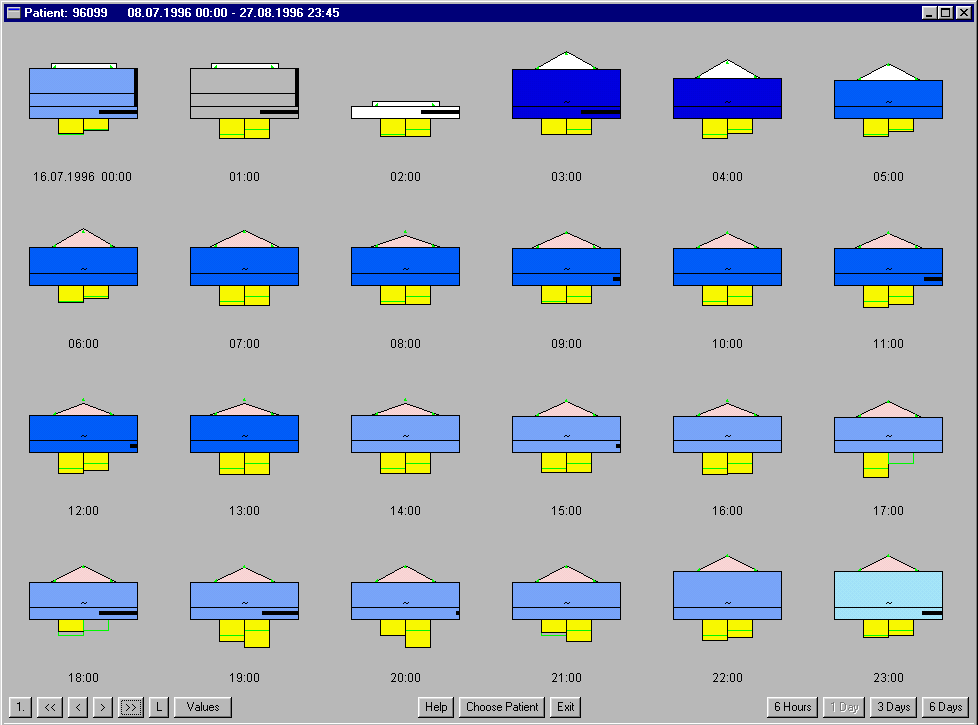
\includegraphics[width=\textwidth]{images/vieVisu.png}
\caption{VIE-VISU is a glyph based visualization for displaying patient vitals~\cite{Horn1998}.}
\label{fig:vieVisu}
\end{figure*}

In some interface implementations, it is conceivable that this connection could be accomplished based on the spatial relationships between prototypes.
For example, placing the left side of one prototype next to the right side of another prototype could trigger a connection between the respective data and property of the primitives.
This visual method of defining connections only works for some spatial relationships. Relationships between color, line weight, or other more abstract spatial properties (area for example) would have to be defined using another interface.

\bodysubsection{Axes and Layout}
\label{axesLayout}

Spatial layout is an important aspect of visualization design.
Administrative data is one of the most common sources of data that influences layout.
For example, in a bar chart, the only actual data on the chart is the vertical height of the bars.
Their horizontal positions come from a sequence, and their vertical position comes from a constant.
The majority of the layout control comes from the step size in the sequence, and the constant mapped to bar width (Figure~\ref{fig:layout}).

\begin{figure*}[t]
\centering
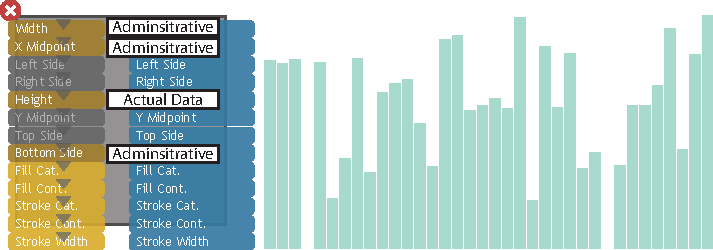
\includegraphics[width=\textwidth]{images/layout.pdf}
\caption{Layout of a bar chart is defined mostly by administrative data.}
\label{fig:layout}
\end{figure*}

The system is limited to layouts that are non-iterative, and do not require spatial information from the layout.
This means that visualizations like tree-maps are not possible, because they subdivide a total space.
This subdivision requires knowing the extents of the total, and iteratively dividing it based on the data.
Word clouds also require iterative layout calculations using information about what is already drawn on the screen.
This feedback loop is not present in the visualization primitives model, as it would require a pipeline approach to achieve.

Axes are not in our current implementation (axes weren't critical for testing creativity), but an axis primitive could provide the labeling necessary.
Its properties would include the label data source, direction, size, etc.
The type of axis could also be driven by a property, switching between a spatial axes or color scale.
The actual labeling could be automatically handled using the extension of Wilkinson's Algorithm by Talbot et al.~\cite{Talbot2010}

Axes are less of an issue for glyphs; the size and position of the objects is entirely relative, there is no axis to compare the spatial dimensions to.
In the case of multiple views (small multiples, trellis displays) that have axes in common, scales exchange information so they can use the same transforms.
This exchange is possible using the output data from each primitive to create connections between the axes present in a visualization.
\bodychapter{EXAMPLES}
\label{examples}

In order to help explain the property mapping process, we present an introduction to the interface, followed by a few examples.

The interface (Figure~\ref{fig:interface}) has four main components.
The left side contains a list of all of the data dimensions loaded into the tool.
The green figures at the top of the screen are buttons for creating new primitives.
In Figure~\ref{fig:interface}, the circle on the right side with the lists of items is a prototype circle primitive.
The golden list on the left side of the circle is the input properties, and the blue list on the right side is the output data from the primitive.
The triangles above each property are scale handles.

Mousing over each property shows the current scale value, and if the property is mapped, highlights the data field that the property is connected to (in this case, area is connected to EmploymentRate).
The grayed out properties are not available because area is mapped, and through the internal geometric relationships that defines the radius and circumference of the circle.
Property mappings are accomplished by clicking on any blue data buttons, and then clicking on any gold property buttons.
Scaling of a mapped property is accomplished by clicking and dragging the triangular handle left or right.

The blue circles are the instances of the primitive that are being specified by the prototype circle.
Together they show the visualization that is produced by the mappings of the prototype.
To prevent occlusion of the visualization, the prototype can be moved around the canvas area by clicking and dragging.
The visualization itself can also be moved around the canvas to help keep all instances on screen (in the case of extremely high or low values).
Dragging the visualization will move all instances of all primitives as a group, in order to keep the data defined relationships intact.
(To try the interface yourself, you may visit~\url{http://visualizationprimitives.net}.)

\begin{figure*}[t]
\centering
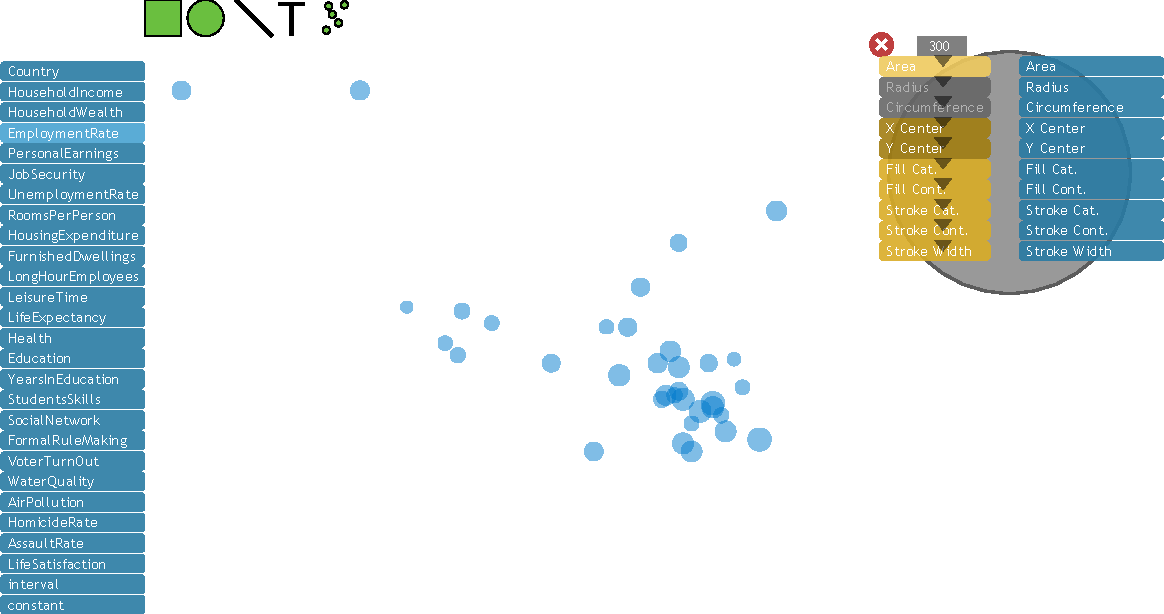
\includegraphics[width=\textwidth]{images/interface.pdf}
\caption{The interface for the current implementation of Visualization Primitives.}
\label{fig:interface}
\end{figure*}

The following examples show how to construct existing familiar visualization types.
Some of them show interesting concepts that are highlighted when producing visualizations from a primitives based approach.
Along with the description of how to construct them, we present versions of each visualization created with our current implementation of visualization primitives.

\bodysection{Bar Chart}
\label{barChart}

Bar charts are created with a rectangle primitive.
In a bar chart, the rectangle only has one data driven visual property, height.
The rectangle's other properties are all derived from administrative data.
Horizontal position is tied to a sequence, while other properties are all tied to a constant.

To create a stacked bar chart, a new rectangle primitive can be connected to the existing rectangle primitive (Figure~\ref{fig:stackedBar}).
To make the connection, the top side of the original rectangle is used as the input for the bottom side of the new rectangle.
They share the same horizontal positions and widths, and the height comes from a separate data source.
Users design not only the prototype primitive, but also the relationships between the prototype primitives.

To create a grouped bar chart, the data assignments are similar (Figure~\ref{fig:groupedBar}).
The two rectangles share the same bottom side position, and the same width, and the height of the new rectangle still comes from external data.
But now the left side of the new rectangle is connected to the right side of the original rectangle.

\begin{figure*}[t]
\centering
\hfill
\subfigure[Stacked Bar Chart]{
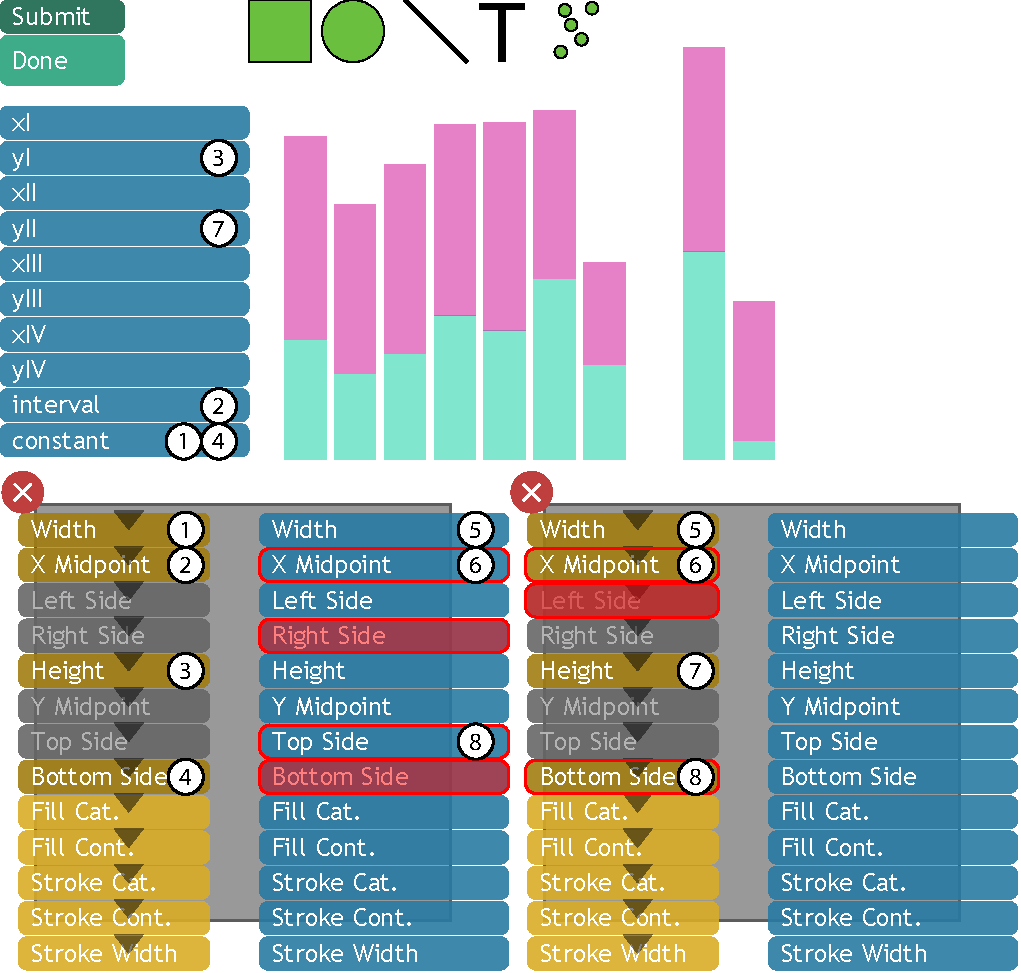
\includegraphics[width=.4\columnwidth]{images/stackedBar.pdf}
\label{fig:stackedBar}
}
\hfill
\subfigure[Grouped Bar Chart]{
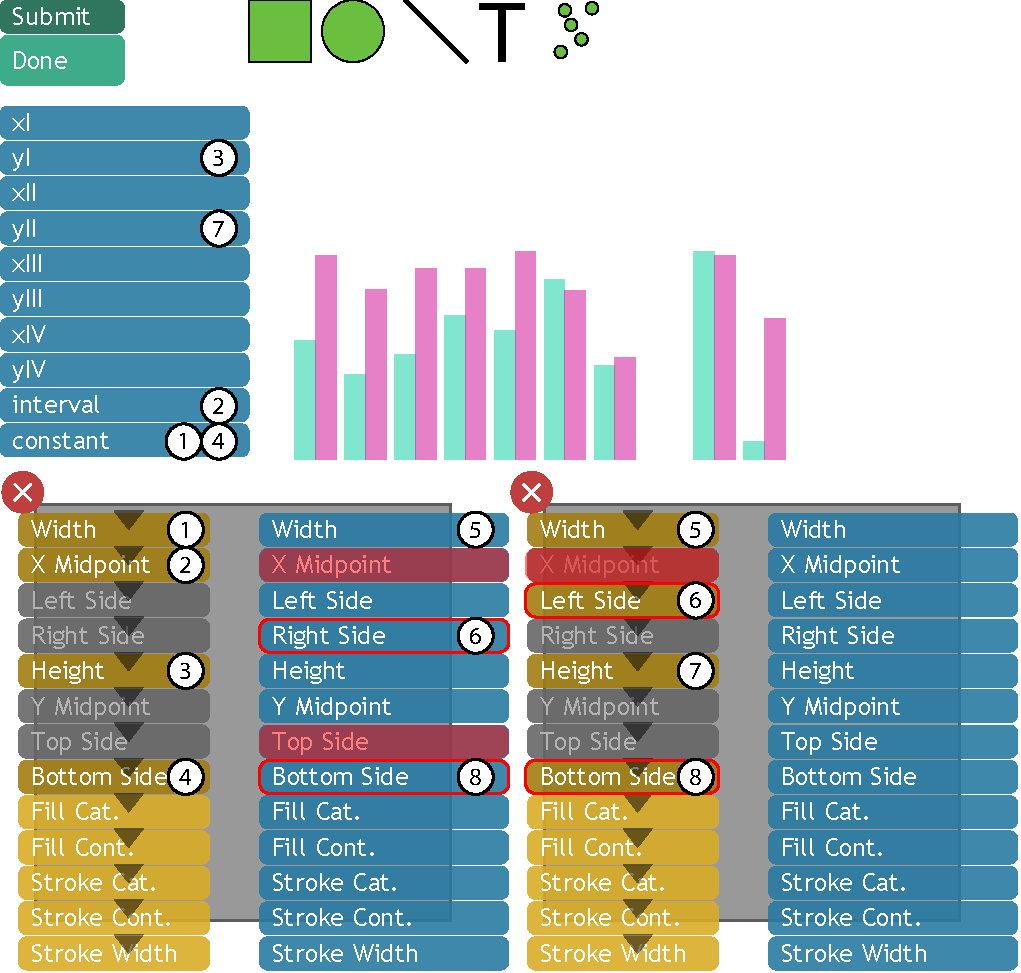
\includegraphics[width=.4\columnwidth]{images/groupedBar.pdf}
\label{fig:groupedBar}
}
\caption{A stacked bar chart and grouped bar chart in our implementation.
The data in both is from Anscombe's Quartet~\cite{Anscombe1973}.
Stacked bars (a) and grouped bars (b) differ only in the mapping of their sides.
The numbers are added to indicate mappings, in the interface mouseover provides this information.
The red highlights indicate the differences in the mappings between the two charts.
}
\label{fig:barCharts}
\end{figure*}

\bodysection{Scatterplot}
\label{scatterplot}

A standard scatterplot showing only one category is easily created with a circle primitive.
Horizontal and vertical position of the shape are the two data driven properties.
The other properties are all administrative.
For some datasets, a scatterplot can represent additional values with the color or size properties.

Scatterplots are very simple to create with our implementation (Figure~\ref{fig:scatterplot}).
In this example a circle has been used, but any primitive in our implementation has the horizontal and vertical position properties that are necessary.
Connecting a categorical value (in this example, number of cylinders) to the fill color property, maps the value to a member of a categorical color scale.

Other primitives designed for scatterplots could provide a categorical visual variable of shape.
This variable would provide access to a set of shapes for representing categorical data.

\begin{figure*}[t]
\centering
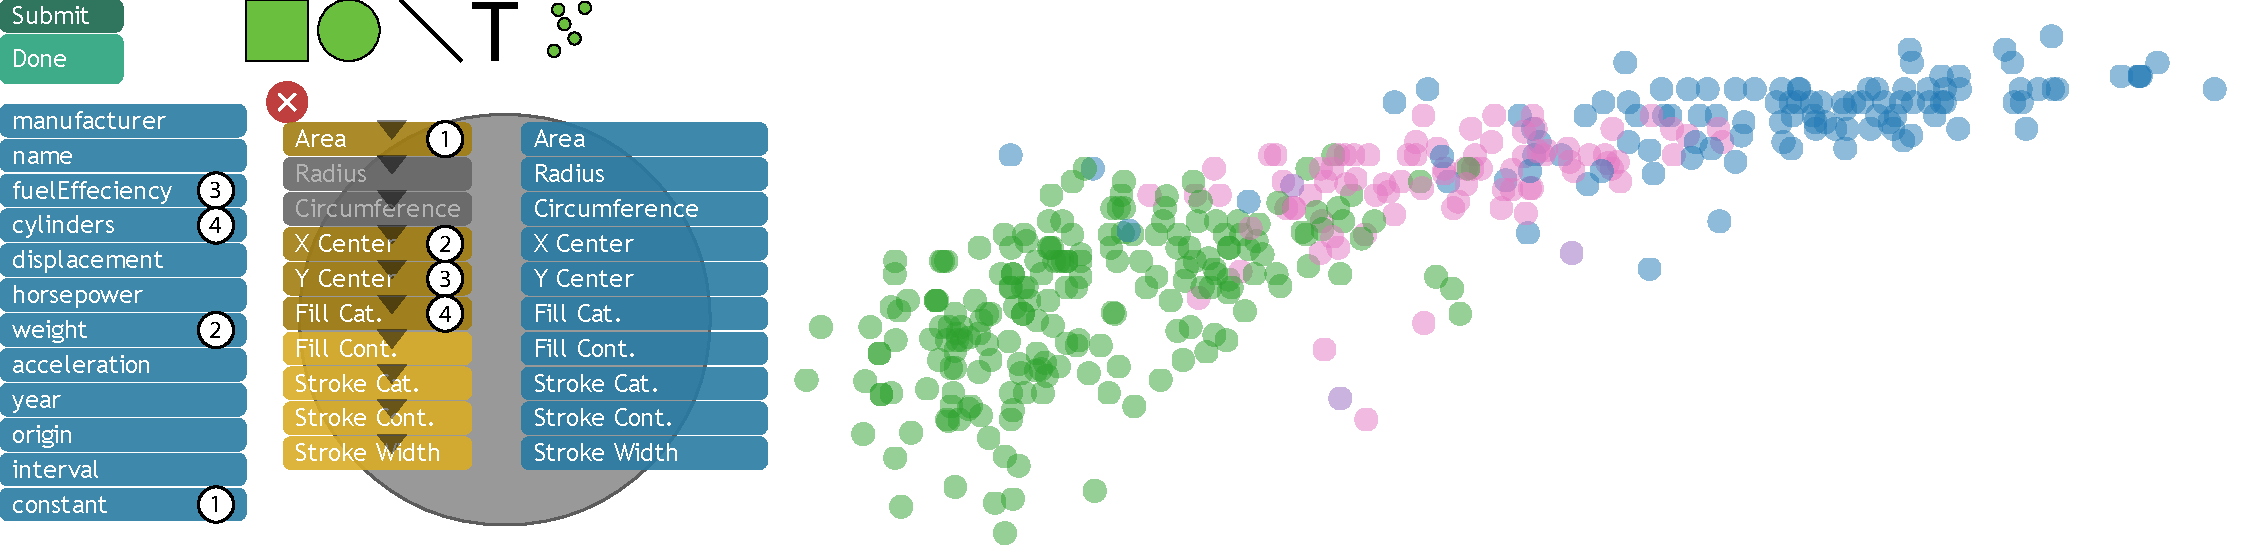
\includegraphics[width=\textwidth]{images/scatterplot.pdf}
\caption{A scatterplot in our implementation using the UCI cars dataset.
Miles per gallon is attached to vertical position, weight is attached to horizontal position.
Number of cylinders is connected to color.
The numbers are added to indicate mappings, in the interface mouseover provides this information.
}
\label{fig:scatterplot}
\end{figure*}

\bodysection{Line Chart}
\label{lineChart}

Line charts are a unique case.
They break the information visualization model slightly by indicating continuity within a data dimension.
This special case requires special treatment in the visualization primitives model.

Line charts need to have the iteration of some of their data to be offset by one.
This makes the two endpoints of the line instances refer to different items in the data, and creates the visual continuity between each data item.
Without this connection, a line chart would simply be a series of points.

There are a number of ways this can be accomplished in the visualization primitives model.
Since a line chart without connections decomposes into points, we opted to make the points primitive allow connections between each point instance.
This allows the line primitive to keep an angular property for creating texture effects.

In a line chart, just like a bar chart, the primitive has one essential visual property.
The remaining properties are all administrative, and only serve to create the layout.

For point primitives in our implementation, the connectedness of the points is also a property.
This allows connections to be driven by data, although in a line chart, connections are mapped to a constant value to turn them on for all instances (Figure~\ref{fig:lineChart}).
When the point primitive draws its instances in the visualization view, it grabs the position for the connection's other end from its previous sibling in the data.
In our current implementation, this uses the existing order of data, however future implementations will include ways to sort data by any of the data dimensions.

\begin{figure*}[t]
   \centering
   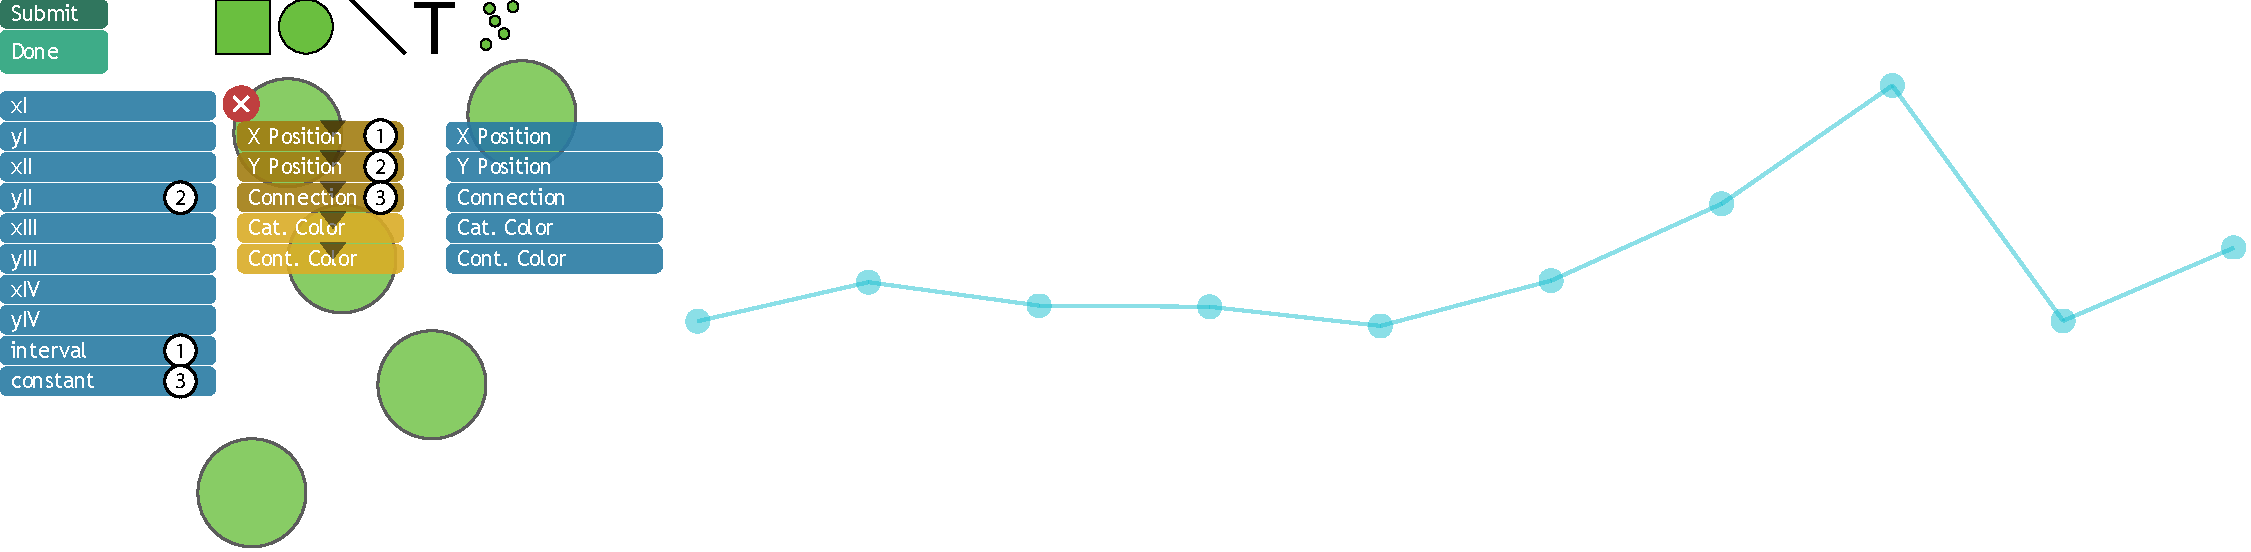
\includegraphics[width=\textwidth]{images/lineChart}
   \caption{
   A line chart in our implementation is created by turning on a connection between points.
   The numbers are added to indicate mappings, in the interface mouseover provides this information.
}
   \label{fig:lineChart}
\end{figure*}

\bodysection{Heat Maps}
\label{heatMap}

Periodic data is often represented in heat map grids where color is tied to data, while time data build the grid (Figure~\ref{fig:heatMap}).
With the right breakdown of time in the data, this is also a simple visualization to create with visualization primitives.
Our example uses Typical Meteorological Year 3 data for Charlotte, NC~\cite{wilcox2008users}.
One data field indicating day of the year is mapped to the vertical position, while horizontal position comes from the hour of the day.
The width and height of the primitive instances comes from a constant value.
The color scale is tied to the dry bulb temperature.
\begin{figure}[t]
   \centering
   \includegraphics[width=.5\columnwidth]{images/heatMap}
   \caption{
   A heat map of temperature using TMY3 data~\cite{wilcox2008users}.
   The numbers are added to indicate mappings, in the interface mouseover provides this information.
}
   \label{fig:heatMap}
\end{figure}

\bodysection{Waterfall Chart}
\label{waterfallChart}

Related to the gantt chart, a less well known chart is the Waterfall Chart (Figure~\ref{fig:presidents}).
This chart type is useful for seeing trends in timeline data.
In our implementation, the chart is created using three primitives showing data on United States Presidents.
One rectangle primitive shows the lifespan of the presidents.
The left side is mapped to birthday, the right side is mapped to the day of their death (or the current date).
The height is assigned a constant value, and the vertical position is a sequence.
Another rectangle primitive displays the presidents' time in office.
The left side is mapped to their inauguration, while the right is mapped to the end of their term.
The height and vertical position come from the respective outputs on the other rectangle primitive.
A text primitive labels the names of each president.
The text string is mapped to the names field.
The left side comes from the right side of the lifespan rectangle, while the vertical position and height are mapped to the respective properties of the lifespan rectangle.
\begin{figure*}[t]
   \centering
   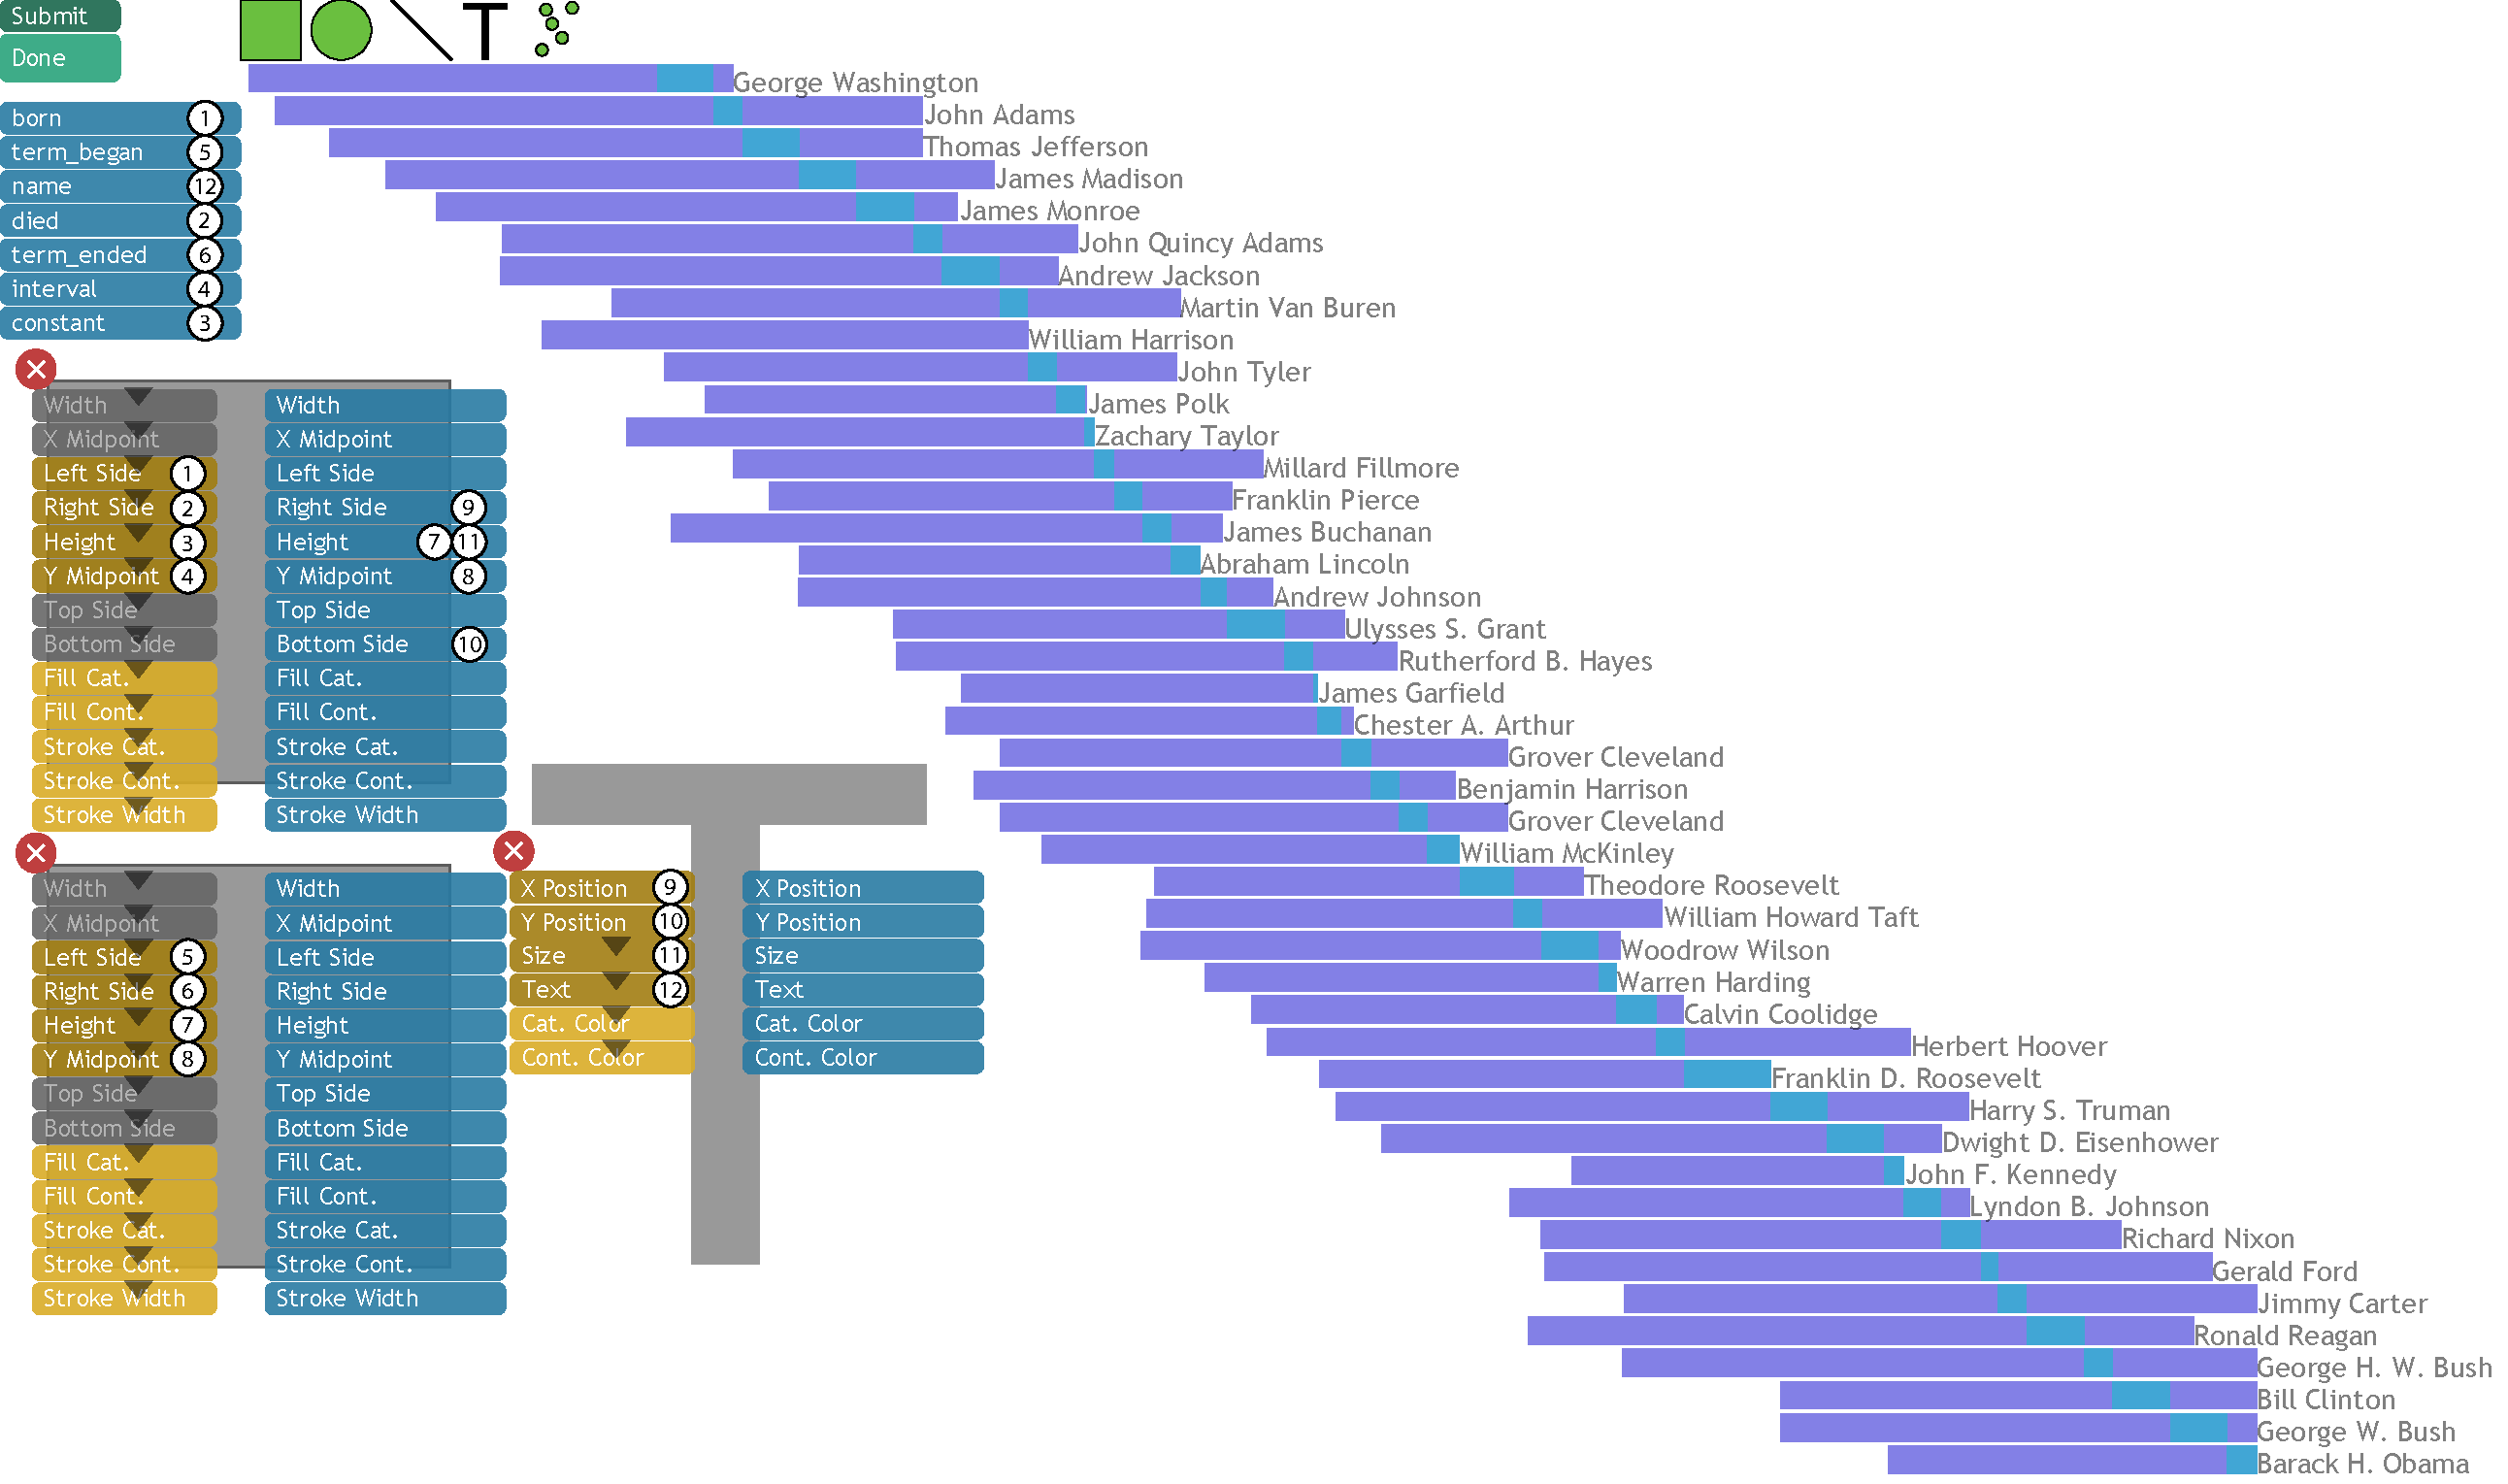
\includegraphics[width=\textwidth]{images/presidents}
   \caption{
   A waterfall chart showing the lifespans and terms of the presidents of the United States.
   The numbers are added to indicate mappings, in the interface mouseover provides this information.
}
   \label{fig:presidents}
\end{figure*}

\bodysection{Glyphs}
\label{glyphs}

Glyphs~\cite{Horn1998} are often used to create small multiples for comparison.
An example of this technique implemented in our system can be seen in Figure~\ref{fig:cars}.
The visualization is built using the cars dataset.
This visualization is not an existing chart type, but is an example of a novel visualization created using visualization primitives.
Four primitives make up each glyph, with each primitive representing a dimension of the data.
Horsepower is the width of the blue rectangles, fuel efficiency is the width of the green rectangles.
The yellow-green ``wheels'' show weight, while the blue ``wheels'' show acceleration.

\begin{figure}[t]
\centering
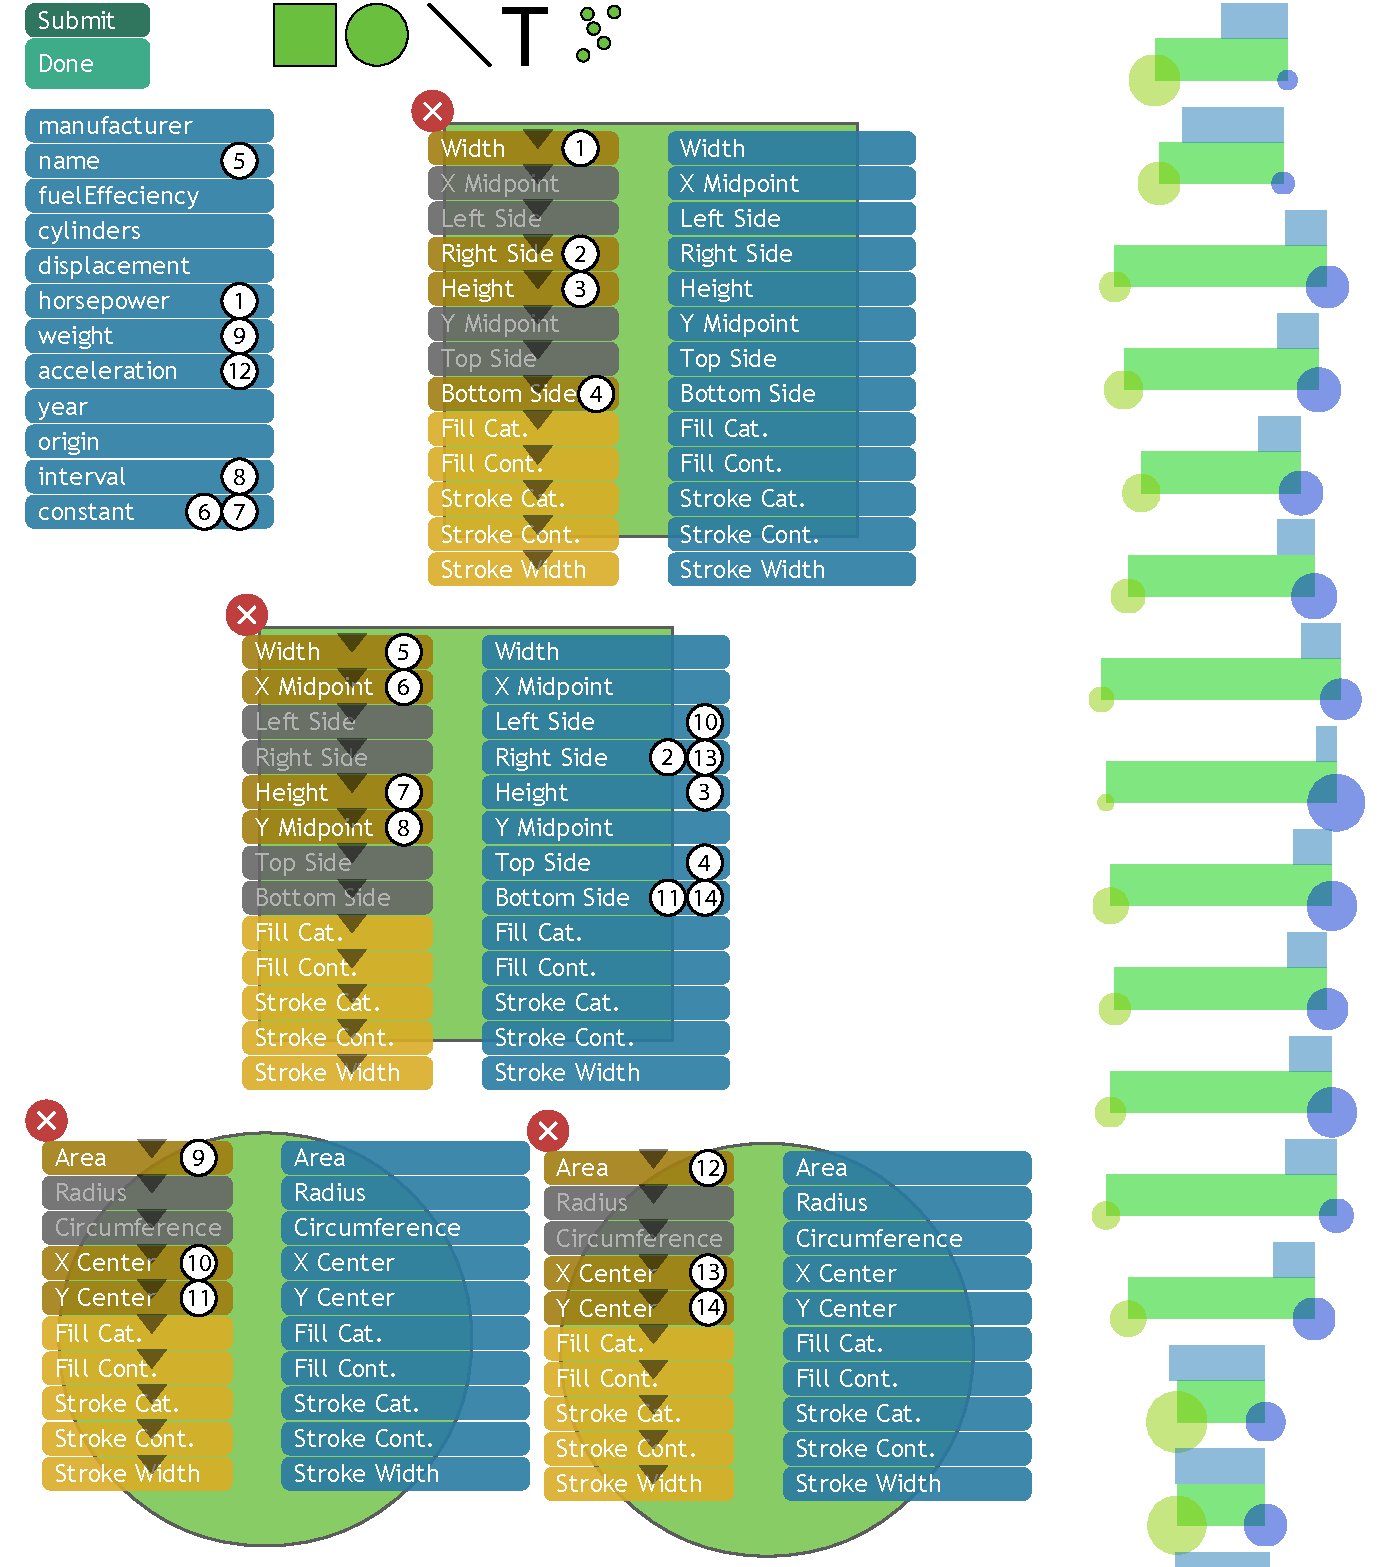
\includegraphics[width=.5\columnwidth]{images/cars.pdf}
\caption{
A glyph technique in our implementation using the cars dataset. The technique is similar to the one used in VIE-VISU~\cite{Horn1998}.
The numbers are added to indicate mappings, in the interface mouseover provides this information.
}
\label{fig:cars}
\end{figure}
\bodychapter{EXPERIMENT}
\label{experiment}

One aim of the visualization primitives model is to enable creativity during the creation of data visualizations.
Given this goal, tests to measure the implementation need to evaluate the ability of the tool to support creativity.
This means that a user study will not evaluate visualization primitives against other tools using tests of task efficiency, or other similar metrics.
Instead, we employ the Creativity Support Index (CSI)~\cite{carroll2009creativity} to evaluate the tool's ability to support creativity.

CSI scores are an index out of 100.
The value is intended to provide a summation of a tool's ability to support creativity.
Along with the indexed score, there are ranked pairs that are also useful for ranking individual components of a tool's creativity support.
For example, support of exploration, effort vs. reward tradeoff, engagement, etc.
The CSI is based closely on a tool�s ability to support a �flow state� for the user.

The study is intended to measure the tool's ability to support creativity, not to quantify the quality of visualizations that are produced.
These concepts are related, however they are not identical.
Creative results are not guaranteed even with tools that support creativity perfectly.
Creativity depends on several components, including the mind of the creator, and the capabilities of the tool at hand.
We have included examples of ``creative'' visualizations generated with visualization primitives, however, these are anecdotal.
Evaluating how creative they are is a secondary issue to how well visualization primitives support creativity.

Tasks that ask a user to find a certain thing in the data could provide inspiration, but they could also constrain thought processes.
Time limits impose pressure that could help or hinder the creative thought process.
We have opted to remove external pressures in the study, allowing participants to build visualizations at their own pace, setting their own tasks along the way.

To test the ability of Visualization Primitives to support creativity in visualization design, we conducted an online experiment. 
We chose an open-ended session design in which participants used Visualization Primitives freely, but with a dataset chosen by the experimenters and with questions preceding and following the session.

Specifically, we formed the following hypotheses regarding Visualization Primitives and creativity:
\begin{itemize}
    \item More experience in visualization would lead to a higher score in the Creativity Support Index.
    \item More experience in visualization would lead to more visualizations generated using the tool.
    \item Visualization Primitives can significantly impact creativity in visualization design for users with sufficient experience with visualizations.
\end{itemize}

\bodysubsection{Materials}
\label{materials}

% can re-order these elements if needed
The materials used in this experiment consist of three main elements: the dataset, visualization-specific demographics, and the Creativity Support Index.

We chose to use the Better Life Index~\cite{url:bli} as a dataset for several reasons.
Primarily, the dataset has been used previously for a creative flower based visualization~\cite{url:bli}.
The dataset is also socially relevant since it contains information on several different countries.
This means a wider group of people may find the data relevant to themselves, encouraging participation.
Finally, the dataset size is large enough to provide interesting possibilities for visualization and analysis, yet small enough to run well in a browser.

Besides typical demographics such as age, education, and gender, we also included questions to measure participants' experience level with visualization tools.
Specifically, participants were asked to rank their experience with other data visualization tools (using a 20-point scale), and to describe their experiences in a text area.

The CSI is an analogue to the NASA Task-load Index (TLX), but for measuring how well a tool supports creativity~\cite{carroll2009creativity}.
In the CSI, participants are first given six 20-point Likert-scale questions that measure the tool's ability to support exploration, collaboration, engagement, expressiveness, perceived effort, and the tool's ability to become transparent to the design process.
Next, participants answer fifteen ranked-pair questions, choosing which of the aforementioned aspects was more important to them during the activity (e.g. exploration versus collaboration).
The CSI questions are shown below.

These questions are answered using a 20-point Likert-scale for each.

\begin{itemize}
	\item It was easy for me to explore many different options, ideas, designs, or outcomes without a lot of tedious, repetitive interaction.
	\item I was able to work together with others easily while doing this activity.
	\item I was very absorbed/engaged in this activity - I enjoyed it and would do it again.
	\item What I was able to produce was worth the effort required to produce it.
	\item While I was doing the activity, the tool/interface/system "disappeared," and I was able to concentrate on the activity.
	\item I was able to be very expressive and creative while doing the activity.
\end{itemize}

For each pair below, please select which factor is most important to you when you were doing this activity.

\begin{tabular}{l l}
Exploration & Collaboration \\
Exploration & Engagement \\
Exploration & Effort/Reward Tradeoff \\
Exploration & Tool Transparency \\
Exploration & Expressiveness \\
Collaboration & Engagement \\
Collaboration & Effort/Reward Tradeoff \\
Collaboration & Tool Transparency \\
Collaboration & Expressiveness \\
Expressiveness & Effort/Reward Tradeoff \\
Expressiveness & Tool Transparency \\
Expressiveness & Engagement \\
Engagement & Tool Transparency \\
Engagement & Effort/Reward Tradeoff \\
Effort/Reward Tradeoff & Tool Transparency \\
\end{tabular}

\bodysubsection{Procedure}
\label{procedure}

Participants were recruited via advertising on Twitter to the URL~\url{http://visualizationprimitives.net}.
No payments or incentives were given.
It took approximately six days to gather all responses.

After following the link, participants were shown a briefing which described the experiment as an open-ended visualization creation tool.
When participants indicated they were ready, they were asked for basic demographics (age, gender, education level).

After completing the demographics, a multiple step tutorial was started.
In this tutorial, participants were required to perform the actions necessary to make a bubble chart (Figure~\ref{fig:tutorialChart}).
Participants were also instructed to submit ``results they were happy with'' at any time via a submit button. That sent their current screen configuration to our server as a SVG (scalable vector graphics) file.

\begin{figure}[t]
\centering
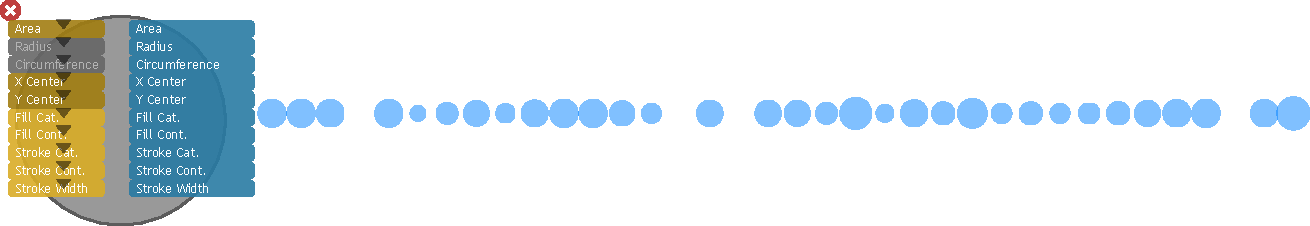
\includegraphics[width=\columnwidth]{images/tutorialResult.pdf}
\caption{
The bubble chart users were left with after completing the tutorial.
}
\label{fig:tutorialChart}
\end{figure}

Following the tutorial, participants were allowed to use Visualization Primitives with the OECD's Better Life Index~\cite{url:bli} dataset for any amount of time, submitting notable visualizations as desired.
In addition to participant-submitted visualizations, the system also auto-submitted when any new mapping was assigned.

When participants indicated they were finished with the open-ended session, they clicked a done button and were presented with the final questionnaire, which contained three parts: visualization-experience, the Creativity Support Index~\cite{carroll2009creativity}, and a space for any additional comments.

\bodysubsection{Results}
\label{results}

As with many online studies, participation drastically fell off with each step.
875 participants made it past the introduction page.
674 answered the demographic information.
95 participants completed the tutorial.
The tutorial was considered a necessary component because without it, the users were not fully introduced to the tool's features.
Of those who completed the tutorial, 44 completed the CSI, and only 31 of those built anything beyond the tutorial before answering the CSI.
Those 31 participants made an average of 14 (median of 8) mappings.
Participants who did not answer the CSI, but completed the tutorial, made an average of 9 (median of 6) mappings.
For the participants who answered the CSI, their average time with the primitives was 21 minutes, with a median of 13, and standard deviation of 23.
Not including submissions made during the tutorial, a total of 1060 SVG files were generated.

Since each participant worked with the same dataset and answered the same questions, our experiment adhered to a between-subjects design for the CSI evaluation.
We divide our analysis into two cases to examine the relationship between experience, perceived creativity support, and productivity (i.e., the number of visualizations produced).

%XXXXX Don't just report CSI results, also number of participants, total number of submissions, submissions per participant, etc.

We excluded 4 participants who did not complete the CSI due to technical issues, and 3 participants who provided meaningless answers for the final questionnaire resulting in $n = 23$ for the final analysis.

%XXXXX What does that mean?
%XXXXX Also, why only 23? I thought we had 45?

Participants were then divided according to their reported experience with visualization tools.
Since a 20-point scale was used for the visualization experience question, we divided participants evenly into a high ($experience >= 17, n = 12$) experience group and a low ($experience < 17, n = 11$) group.

\begin{figure}[t]
    \subfigure[Collaboration]{
        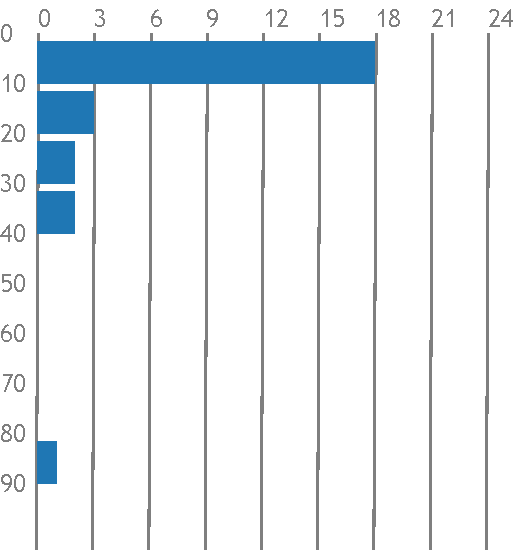
\includegraphics[width=.3\columnwidth]{images/histograms/collaboration.pdf}
        \label{fig:collaboration}
    }
    \hfill
    \subfigure[Engagement]{
        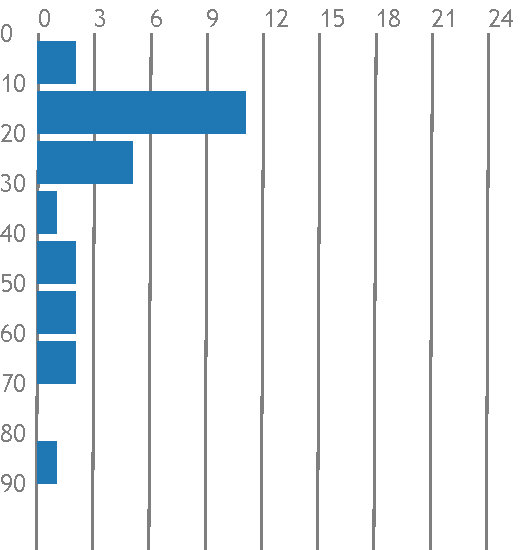
\includegraphics[width=.3\columnwidth]{images/histograms/engagement.pdf}
        \label{fig:engagement}
    }
    \hfill
    \subfigure[Exploration]{
        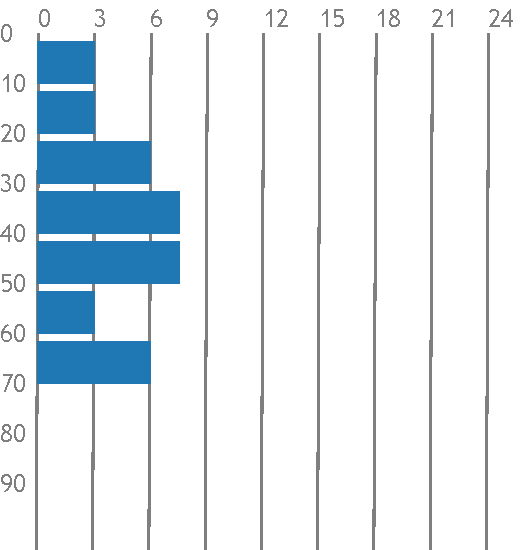
\includegraphics[width=.3\columnwidth]{images/histograms/exploration.pdf}
        \label{fig:exploration}
    }
    \hfill
    \subfigure[Expressiveness]{
        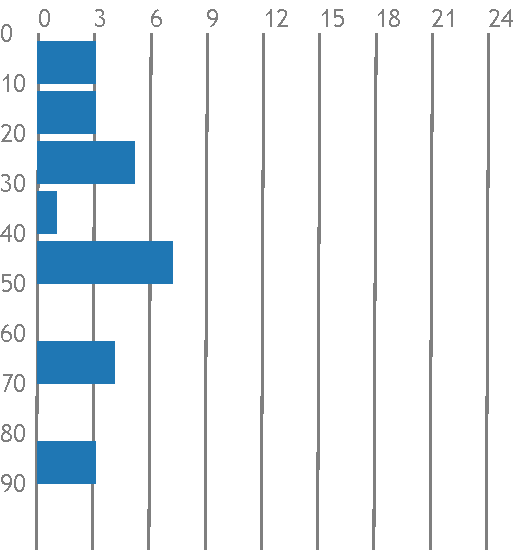
\includegraphics[width=.3\columnwidth]{images/histograms/expressiveness.pdf}
        \label{fig:expressiveness}
    }
    \hfill
    \subfigure[Effort/Reward]{
        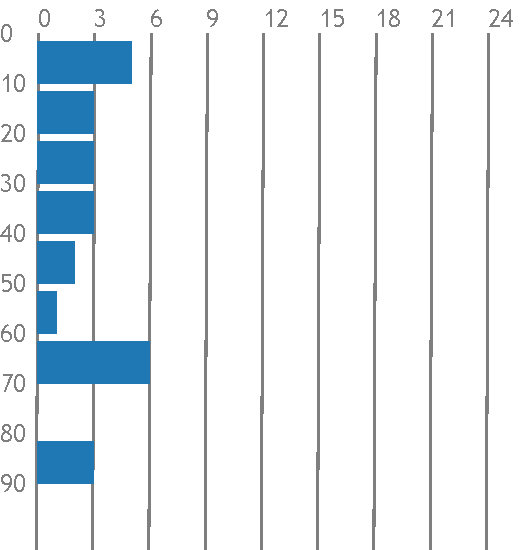
\includegraphics[width=.3\columnwidth]{images/histograms/tradeoff.pdf}
        \label{fig:tradeoff}
    }
    \hfill
    \subfigure[Tool Transparency]{
        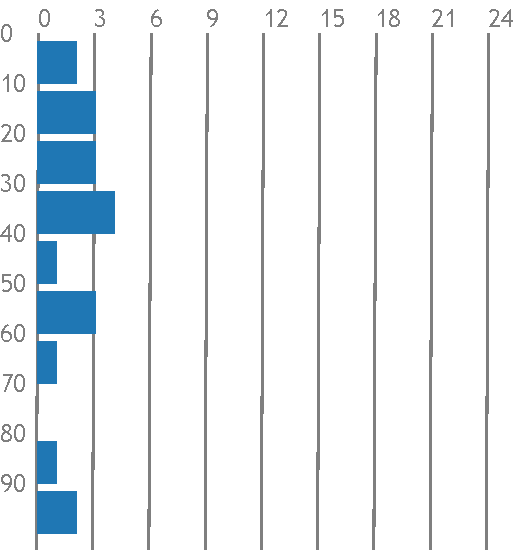
\includegraphics[width=.3\columnwidth]{images/histograms/transparency.pdf}
        \label{fig:transparency}
    }
\caption{Histograms of the rankings for each factor
(built using the visualization primitives prototype).}
\label{fig:histograms}
\end{figure}


\bodysubsubsection{Experience and Creativity Support}
\label{experienceAndCreativitySupport}

CSI scores are an index out of 100.
They are calculated by combining ranked pairs with Likert scale results.
For each factor, the Likert scale results are multiplied by the total factor count from the ranked pair portion.
This value is then added to all the other factor results, and divided by 3 to arrive at an index out of 100.
Table~\ref{table:factorRankings} and Figure~\ref{fig:histograms} show the CSI results for our experiment.

\begin{table}
    \centering
        \begin{tabular}{l|r|r|r}
            Factor�������� & Mean� & Median & Standard Deviation \\         \hline
            exploration��� & 41.62 & 39.5�� & 24.46������������� \\ 
            collaboration� & 9���� & 0����� & 18.22������������� \\ 
            engagement���� & 26.31 & 18.5�� & 19.87������������� \\ 
            tradeoff������ & 37.73 & 37.5�� & 27.3�������������� \\ 
            transparency�� & 53��� & 45���� & 35.48������������� \\ 
            expressiveness & 38.23 & 40���� & 23.52������������� \\
        \end{tabular}

    \caption{\label{table:factorRankings} Factor ranking results.}
\end{table}

\begin{figure*}[p]
    \subfigure[]{
        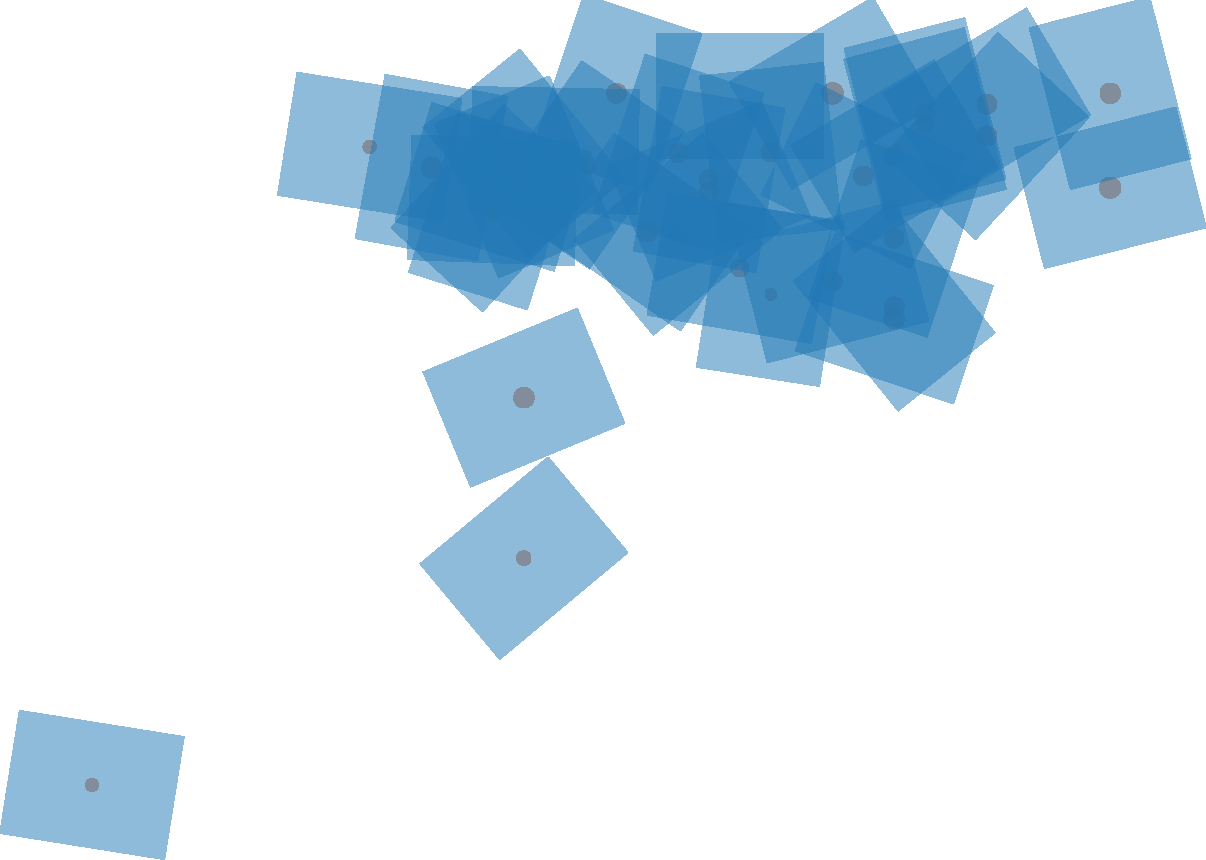
\includegraphics[width=200pt]{images/gallery/svg-lCMWzs3C-77-auto2.pdf}
        \label{fig:gallery7}
    }
    \hfill
    \subfigure[]{
        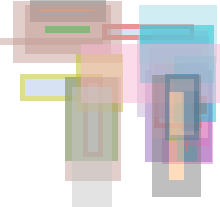
\includegraphics[width=160pt]{images/gallery/svg-iBaorUUg-69-auto2.pdf}
        \label{fig:gallery4}
    }
    \hfill
    \subfigure[]{
        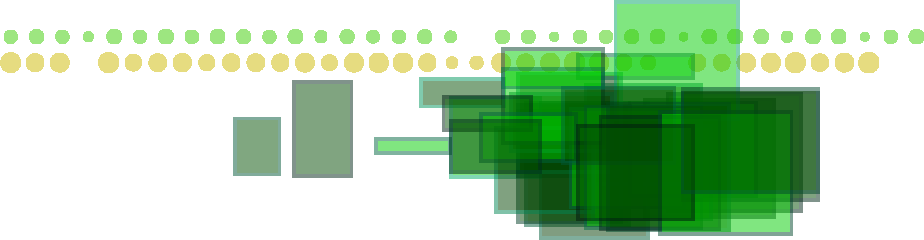
\includegraphics[width=.45\columnwidth]{images/gallery/svg-HKI5oDTV-30-auto2.pdf}
        \label{fig:gallery3}
    }
    \hfill
    \subfigure[]{
        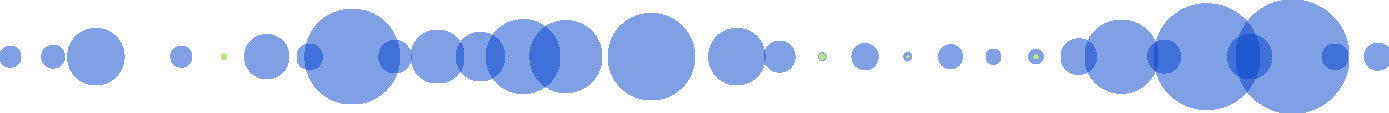
\includegraphics[width=.45\columnwidth]{images/gallery/svg-kJfnjNbc-4-auto2.pdf}
        \label{fig:gallery5}
    }
    \hfill
    \subfigure[]{
        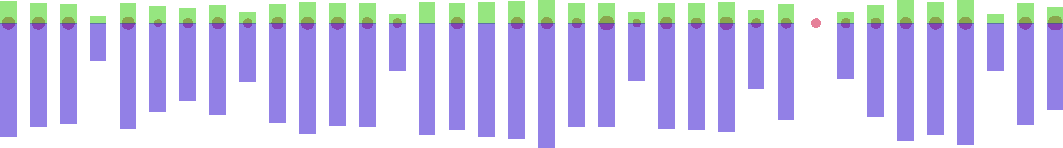
\includegraphics[width=.45\columnwidth]{images/gallery/svg-lCMWzs3C-26-auto2.pdf}
        \label{fig:gallery6}
    }
    \hfill
    \subfigure[]{
        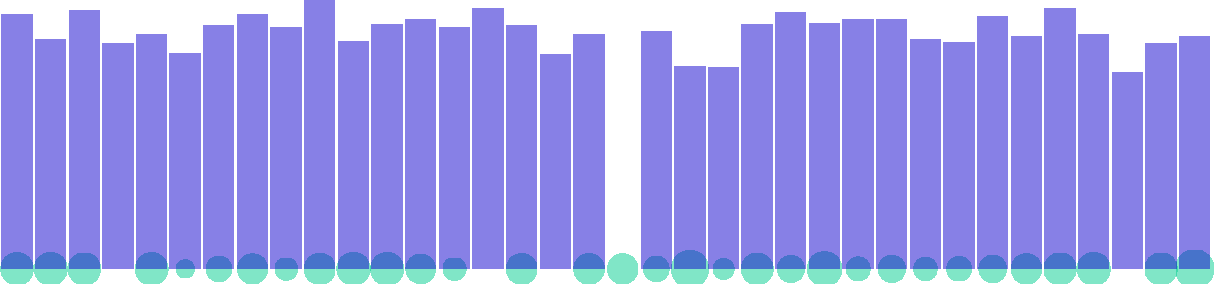
\includegraphics[width=.45\columnwidth]{images/gallery/svg-UBDlMBE2-29-auto2.pdf}
        \label{fig:gallery8}
    }
    \hfill
    \subfigure[By the same participant as \ref{fig:gallery1}.]{
        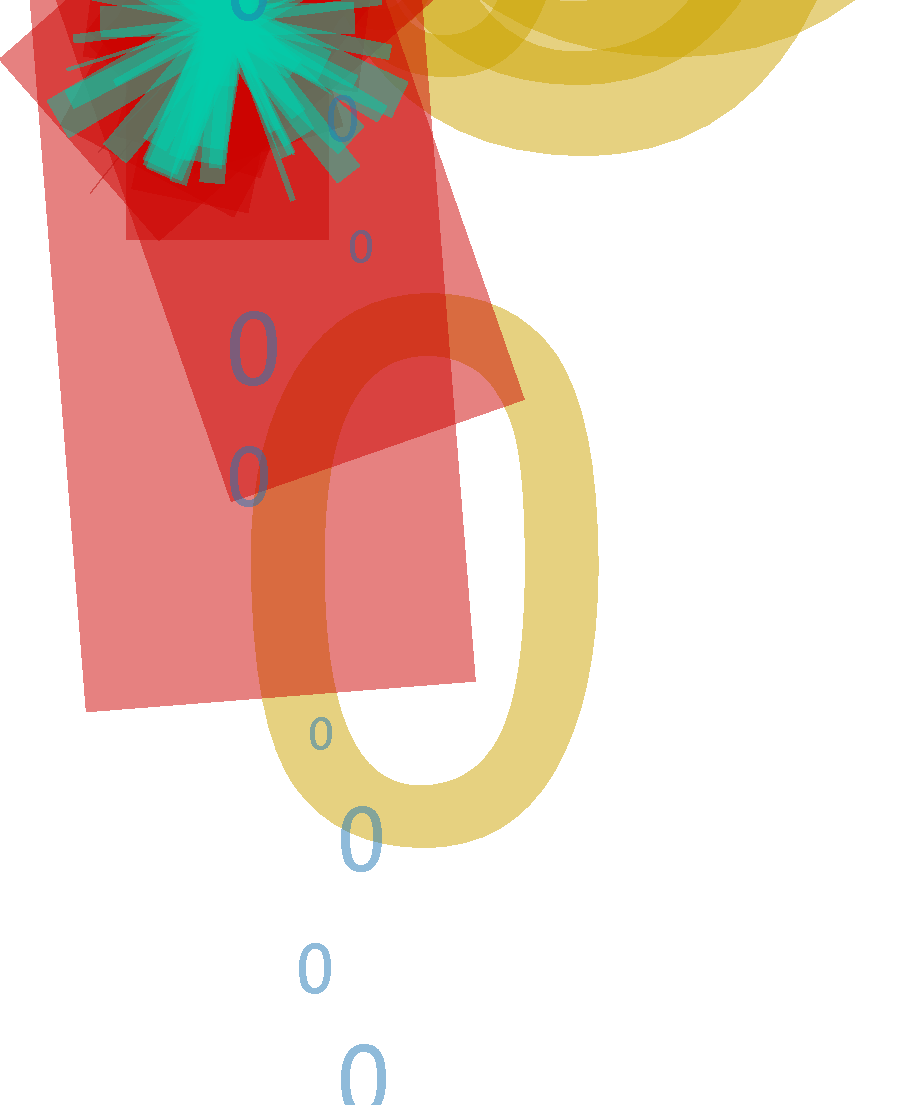
\includegraphics[width=.45\columnwidth]{images/gallery/svg-47GM6Lk3-87-auto2.pdf}
        \label{fig:gallery2}
    }
    \hfill
    \subfigure[By the same participant as \ref{fig:gallery2}.]{
       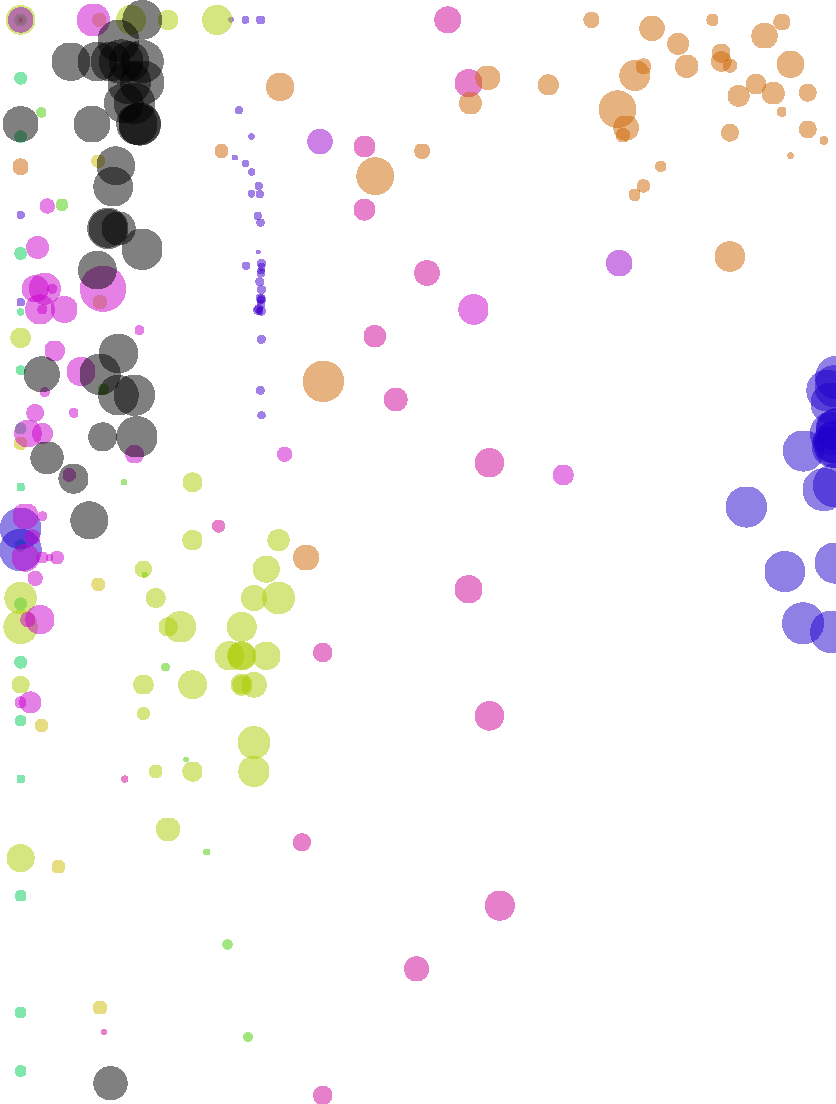
\includegraphics[width=.45\columnwidth]{images/gallery/svg-47GM6Lk3-61-auto2.pdf}
       \label{fig:gallery1}
   }
\caption{A selection of example visualizations submitted by study participants.}
\end{figure*}

We compared CSI scores for the low-experience and high-experience groups using a t-test.
This yields a significant effect for the CSI-score $t(21) = 2.0843; p = 0.0495$, with CSI-score in the high-experience group being higher than that of the low-experience group. 
The lower mean CSI-score appeared in the low-experience group ($M = 54.27, SD = 22.50$), meaning participants in the high-experience group felt that Visualization Primitives supported their creativity in visualization design more ($M = 73.75, SD = 22.28$).
(The paper presenting the CSI offers a sample ranking of 77.3~\cite{carroll2009creativity})
These results are consistent with our hypothesis that Visualization Primitives can significantly impact creativity in visualization design for participants who have sufficient experience with visualizations.

\bodysubsubsection{Experience and Productivity}
\label{experienceAndProductivity}

We also compared experience with the total number of SVG graphics submitted.
This did not yield a significant effect for the the total number of SVGs submitted, although participants in the high-experience group submitted more SVGs on average ($M = 21, SD = 19$) than those in the low-experience group ($M = 17, SD = 10$). % $t(21) = 0.6745; p = 0.5073$
These results do not support our hypothesis that users with more experience in visualization would submit a higher number of visualizations.

\bodysubsubsection{General CSI Results}
\label{CSIResults}

In addition to discussing the total CSI scores, it is also useful to look at which categories the participants ranked most important to them while using Visualization Primitives.
These results are shown in Figure~\ref{fig:histograms}.
Tool transparency and exploration ranked most important, while collaboration and engagement ranked at the bottom of users' priorities.

\bodysubsubsection{Example Visualizations}
\label{exampleVisualizations}

The vast majority of users generated simple visualizations with a single primitive.
Since the tutorial left users with a circle primitive, scatterplots became one of the most common visualizations that was created.
Many users created visuals with only one or two primitives, and often there was no data driven spatial relationship between those primitives.
Connections between primitives were rare, possibly because that ability was not explicitly shown to users during the tutorial, only described in text.
The connections that were created were often built off of the bubble chart created during the tutorial (Figures~\ref{fig:gallery6},~\ref{fig:gallery8}).
Often the creations fell somewhere between art and data visualization (Figures~\ref{fig:gallery7},~\ref{fig:gallery3},~\ref{fig:gallery5}), and some resulted in purely artistic work (Figures~\ref{fig:gallery4},~\ref{fig:gallery2},~\ref{fig:gallery1}).
\bodychapter{DISCUSSION}
\label{discussion}

The results of the experiment indicate that visualization primitives support creativity, especially with users who have had adequate experience with visualization tools.

User interface issues were a limiting factor in users' exploration of the design space.
Specifically, having to mouse over properties to see what they were bound to made it difficult to build and maintain a mental model of what was being shown.
While our goal was to reduce clutter from connecting lines, the alternative may have created more issues than it solved.

The unfamiliarity of the interface definitely contributed to many users frustrations.
Many comments expressed users' frustration with not knowing what the parts of the interface did.
This could be addressed by further iterations of the tutorial and improvements to the UI.

The internal geometric representations of the primitives also may have contributed to confusion.
Drawing elements to the screen is often not possible until multiple properties have been specified.
This could be alleviated with default values, however the solution is far from elegant, and can produce unexpected behavior when assigning properties.

Not all the results that participants created and submitted were strictly visualizations in the sense of being useful. We see some playful examples that are more artistic than useful, which is in line with our goals. We did not ask people to create anything in particular so as not to constrain their exploration.

The considerable time spent on the site shows that they were engaged and interested in exploration, despite the user interface flaws.
This suggests that tapping into users' creativity is a promising way of getting them interested in visualization.

\bodysubsection{Lessons Learned}
\label{lessonsLearned}

This experiment was very obviously flawed in many ways, however it revealed to me that there were many components of visualization primitives that need work.
The interface issues became a major hinderance to testing the model, and the experiment design itself needs a lot of improvement.
The best course of action for proceeding is to take what I learned about the interface and spend a significant amount of time improving it.
After the interface has been revisited, the experiments need to be planned to evaluate both the creativity of the product the participants create, and the creativity support of the application.

In addition, the experiments need to provide more direction to the participants.
Rather than a period of free exploration, the participants need to be given a task to achieve.
This constraint should help to focus participants, and will make it possible to evaluate the creativity involved in what they produce. Some possible tasks would be: "Create three visualizations that answer x." or "Show a visualization that answers both x and y."
Still including a period of open exploration before the tasks may help participants to become more familiar with the tool, and make it easier for them to achieve the given tasks later.

Without knowing the purpose the participants had when creating a visualization, it is impossible to rate the usefulness of the visualization, and therefore impossible to evaluate how creative it was.
Providing a task structure to participants means that the usefulness can be evaluated, and even ranked against other participant's produced visualizations.

Evaluating creativity of the participant's product may be best accomplished through the use of the Consensual Assessment Technique (CAT)~\cite{Amabile1996}.
The technique involves a panel of expert judges who spend time examining the "creative" works, and evaluating their creativity.
A panel of three to five judges will be able to rate the creativity of what is created. This information can then be used in conjunction with the Creativity Support Index to better determine the creativity support of the tool, and validate the participant's answers to the CSI.

Another change that should be made to the study is the participant selection. The shotgun approach of attracting random participants on the internet is likely partially responsible for the extremely low completion rate of the study. It also means that many participants were not as familiar with the concept of visualization, so their produced results were more like data art than visualization. Manually recruiting participants can help to constrain the group to individuals who are aware of things like Bertin's hierarchy of retinal variables~\cite{bertin1983semiology}. This will increase the likelihood that their visualizations will be useful for a task.

\bodysubsection{Interface Improvements}
\label{interfaceImprovements}
The visualization primitives model has proven to be effective at some things, however there are still limitations due to the implementation.
The areas that could result in the most striking improvements in creativity support deal with the interface, and are needed mostly to help users achieve a flow state.

\bodysubsubsection{Default Values}
\label{defaultValues}
In the current implementation, there are no default values assigned to any of the properties.
This results in there being no feedback to the user when they map properties that require multiple other properties to also be mapped.
Once the necessary subset of properties has been mapped, the primitive can draw itself, but in the intermediate time, the primitive does nothing.
For example, a rectangle primitive needs two horizontal properties mapped out of four, and two vertical properties mapped out of four.
Without default values, the primitive cannot draw itself until four out of those eight properties have been mapped.

To complicate things further, knowing which properties to assign defaults to depends on the internal geometric relationships of the primitive.
The best way to solve this is probably a decision tree that chooses which defaults to assign based on what else has been assigned already.
The important part of this decision tree structure is how it fits into the internal geometric relationship architecture, and how it gets initiated in the mapping assignment.

Fixing this so that there is always immediate feedback should help the user experience 

\bodysubsubsection{Primitives Graph}
\label{primitivesGraph}
The visualization primitives model allows for dependency relationships to occur between the properties of primitives.
These dependencies are represented through mappings.

Mappings in the current implementation record connections between data output, and a property.
The system for storing them is simplistic, as each only belongs to the parent primitive.
There are currently no methods for traversing the structures of mappings that can be created.
This presents problems with updating child primitives when a parent primitive is modified.

A proper system for storing mappings would allow traversal of the mappings, and prevent circular traversals when a loop is present in the structure.
The current implementation also means that scaling of values is clumsy when those values come from a parent primitive and not the original data.
A better structure would allow the properties to retrieve the scale value from the parent and modify it rather than just multiplying their own scale value on top.

This structure will allow for a better interface and more consistent experience with scaling data inputs to properties.
This should help the user to achieve a flow state by making the interface control behavior more intuitively.

\bodysubsubsection{Connections Between Primitives}
\label{primConnectionsFW}
Currently, the interface provides buttons for each visual property that a primitive has, and output buttons that pass the primitive's data through.
This interface works for testing the model, but it is hardly user-friendly.
Ideally, the interface should feel much more natural, and have the same feeling of direct connections that come from the implementation's immediate feedback.

As mentioned, one possible way to accomplish that is through using the location of the prototypes relative to each other to help determine the spatial relationships between primitives.
This type of connection feels physical, and would be relatively intuitive to users.
However spatial relationships cannot define mappings for properties like color, rotation, or line weight.
These mappings sill need some sort of input and output interface, and may require things like icon representations or other interface elements to allow their mapping.
The interactions of connecting abstract visual properties of different objects are new, and there are not many metaphors to the physical world.
Inspiration for these elements could, however, be drawn from layout or drawing tools.

For example, rotation of an object in many vector drawing programs is accomplished using a handle on the object.
Perhaps using a similar handle for controlling rotation would improve the intuitiveness of the connection process.
Unfortunately, interface elements borrowed from drawing tools may not be intuitive for users that are not familiar with them.
Testing of several different approaches may be necessary to determine what interactions are simplest to grasp and use for most users.

\bodysubsubsection{Set of Primitives}
\label{setPrimitivesFW}
The set of primitives provided by the system has the most profound impact on what can be created with the system.
The current set is definitely not ideal.
Future tweaking of the set should help to optimize the balance between simplicity and flexibility.

One potential way to proceed with this is to build a list of visualizations that fall within the theoretical constraints of the system (tabular data, non-iterative layouts, etc.)
Establishing which visualizations in the list cannot be created with the current set of primitives will help to identify possible primitives that should be created.
It also may be possible to tweak the properties and internal geometric representations of existing primitives to allow the creation of other visualizations.

Identifying which primitives to add, and which to remove (when there is excessive overlap in their capabilities) is the difficult part.
The best way to achieve this may be to select the primitives that cover the greatest range of visualization techniques that are not possible with the current set.
By aiming for the best coverage first, corner cases can be identified, and helpful modifications to existing primitives should be easier to find.

Once the list of theoretically possible visualizations can all be created with the implementation, the implementation will be complete.
This still will not mean that the set of primitives is optimal for a given task, but it does guarantee maximum flexibility of the system.

\bodysubsubsection{Creativity Support}
\label{creativitySupportFW}
The initial evaluation of creativity support had several issues.
Aside from using an earlier version of the CSI, the tutorial teaching people how to use the system probably needed to be enforced better.
Several people didn't finish the tutorial entirely before exploring on their own and continuing the study.
This is a minor issue, and easily fixable in the next study.

It would also be good to provide a task for participants to perform.
The participants of the last study seemed to just play around with the visuals, and not think much about 
A goal will help to focus people and give them constraints to work within.

The difficulty in this task is finding a goal that strikes a good balance between open ended solutions, and providing focus.
If the goal is too open ended, it will not serve as a motivator.
But if the goal is too constrained, there will be a small handful of solutions and no creative solutions will be generated.
One possible way to alleviate this is to pick a more focused goal, and follow it up with a period of free exploration for users to express their creativity.
\bodychapter{FUTURE WORK}
\label{futureWork}
The visualization primitives model has proven to be effective at some things, however there are still limitations due to the implementation.
There are several areas that need to be re-examined in order to further the work and test more of the model.
Many of these areas deal with the implementation of the model, and they will help to round out the capabilities of the tool, and ensure it covers a sufficiently sized design space.
Some of the areas are related more to modifications of the implementation, not directly related to the model.
These modifications will help to improve the overall function, and remove some of the buggier behavior of the implementation.
The areas that could result in the most striking improvements in creativity support deal with the interface, and are needed mostly to help users achieve a flow state.

\bodysubsection{Default Values}
\label{defaultValues}
In the current implementation, there are no default values assigned to any of the properties.
This results in there being no feedback to the user when they map properties that require multiple other properties to also be mapped.
Once the necessary subset of properties has been mapped, the primitive can draw itself, but in the intermediate time, the primitive does nothing.
For example, a rectangle primitive needs two horizontal properties mapped out of four, and two vertical properties mapped out of four.
Without default values, the primitive cannot draw itself until four out of those eight properties have been mapped.

To complicate things further, knowing which properties to assign defaults to depends on the internal geometric relationships of the primitive.
The best way to solve this is probably a decision tree that chooses which defaults to assign based on what else has been assigned already.
The important part of this decision tree structure is how it fits into the internal geometric relationship architecture, and how it gets initiated in the mapping assignment.

Fixing this so that there is always immediate feedback should help the user experience 

\bodysubsection{Primitives Graph}
\label{primitivesGraph}
The visualization primitives model allows for dependency relationships to occur between the properties of primitives.
These dependencies are represented through mappings.

Mappings in the current implementation record connections between data output, and a property.
The system for storing them is simplistic, as each only belongs to the parent primitive.
There are currently no methods for traversing the structures of mappings that can be created.
This presents problems with updating child primitives when a parent primitive is modified.

A proper system for storing mappings would allow traversal of the mappings, and prevent circular traversals when a loop is present in the structure.
The current implementation also means that scaling of values is clumsy when those values come from a parent primitive and not the original data.
A better structure would allow the properties to retrieve the scale value from the parent and modify it rather than just multiplying their own scale value on top.

This structure will allow for a better interface and more consistent experience with scaling data inputs to properties.
This should help the user to achieve a flow state by making the interface control behavior more intuitively.

\bodysubsection{Connections Between Primitives}
\label{primConnectionsFW}
Currently, the interface provides buttons for each visual property that a primitive has, and output buttons that pass the primitive's data through.
This interface works for testing the model, but it is hardly user-friendly.
Ideally, the interface should feel much more natural, and have the same feeling of direct connections that come from the implementation's immediate feedback.

As mentioned, one possible way to accomplish that is through using the location of the prototypes relative to each other to help determine the spatial relationships between primitives.
This type of connection feels physical, and would be relatively intuitive to users.
However spatial relationships cannot define mappings for properties like color, rotation, or line weight.
These mappings sill need some sort of input and output interface, and may require things like icon representations or other interface elements to allow their mapping.
The interactions of connecting abstract visual properties of different objects are new, and there are not many metaphors to the physical world.
Inspiration for these elements could, however, be drawn from layout or drawing tools.

For example, rotation of an object in many vector drawing programs is accomplished using a handle on the object.
Perhaps using a similar handle for controlling rotation would improve the intuitiveness of the connection process.
Unfortunately, interface elements borrowed from drawing tools may not be intuitive for users that are not familiar with them.
Testing of several different approaches may be necessary to determine what interactions are simplest to grasp and use for most users.

\bodysubsection{Set of Primitives}
\label{setPrimitivesFW}
The set of primitives provided by the system has the most profound impact on what can be created with the system.
The current set is definitely not ideal.
Future tweaking of the set should help to optimize the balance between simplicity and flexibility.

One potential way to proceed with this is to build a list of visualizations that fall within the theoretical constraints of the system (tabular data, non-iterative layouts, etc.)
Establishing which visualizations in the list cannot be created with the current set of primitives will help to identify possible primitives that should be created.
It also may be possible to tweak the properties and internal geometric representations of existing primitives to allow the creation of other visualizations.

Identifying which primitives to add, and which to remove (when there is excessive overlap in their capabilities) is the difficult part.
The best way to achieve this may be to select the primitives that cover the greatest range of visualization techniques that are not possible with the current set.
By aiming for the best coverage first, corner cases can be identified, and helpful modifications to existing primitives should be easier to find.

Once the list of theoretically possible visualizations can all be created with the implementation, the implementation will be complete.
This still will not mean that the set of primitives is optimal for a given task, but it does guarantee maximum flexibility of the system.

\bodysubsection{Contextualizing Visualizations}
\label{contextualize}
One possible application of the model is to help contextualize current visualizations.
I would like to use the visualization primitives model to help classify visualizations.
The theoretical constraints of the model closely match many of the core concepts in the InfoVis model, and could provide helpful new ways to categorize existing visualization techniques.

\bodysubsection{Creativity Support}
\label{creativitySupportFW}
The initial evaluation of creativity support had several issues.
Aside from using an earlier version of the CSI, the tutorial teaching people how to use the system probably needed to be enforced better.
Several people didn't finish the tutorial entirely before exploring on their own and continuing the study.
This is a minor issue, and easily fixable in the next study.

It would also be good to provide a task for participants to perform.
The participants of the last study seemed to just play around with the visuals, and not think much about 
A goal will help to focus people and give them constraints to work within.

The difficulty in this task is finding a goal that strikes a good balance between open ended solutions, and providing focus.
If the goal is too open ended, it will not serve as a motivator.
But if the goal is too constrained, there will be a small handful of solutions and no creative solutions will be generated.
One possible way to alleviate this is to pick a more focused goal, and follow it up with a period of free exploration for users to express their creativity.

Despite creativity being a component of what the tool supports, creativity support is not the only goal of the model.
The primary goal of the model is to provide an alternative method to conceptualize visualization creation.
This method could help teach the concept of data visualization, and to help build other tools or toolkits for creating data visualizations.
Evaluating the tool's ability to support creativity is a means to evaluate the model's possibilities.
\bodychapter{FUTURE WORK}
\label{futureWork}
This pass at implementing the visualization primitives model has proven to be effective at some things, however there are still limitations due to the implementation.
There are several areas that need to be re-examined in order to further the work and test more of the model.
Many of these areas deal with the implementation of the model, and they will help to round out the capabilities of the tool, and ensure it covers a sufficiently sized design space.
Some of the areas are related more to tweaks to the implementation, not directly related to the model.
These tweaks will help to improve the overall function, and remove some of the buggier behavior of the implementation.
The areas that could result in the most striking improvements in creativity support deal with the interface, and are needed mostly to help users achieve a flow state.

\bodysubsection{Default Values}
\label{defaultValues}
In the current implementation, there are no default values assigned to any of the properties.
This results in there being no feedback to the user when they map properties that require multiple other properties to also be mapped.
Once the necessary subset of properties has been mapped, the primitive can draw itself, but in the intermediate time, the primitive does nothing.
For example, a rectangle primitive needs two horizontal properties mapped out of four, and two vertical properties mapped out of four.
Without default values, the primitive cannot draw itself until four out of those eight properties have been mapped.

To complicate things further, knowing which properties to assign defaults to depends on the internal geometric relationships of the primitive.
The best way to solve this is probably a decision tree that chooses which defaults to assign based on what else has been assigned already.
The important part of this decision tree structure is how it fits into the internal geometric relationship architecture, and how it gets initiated in the mapping assignment.

\bodysubsection{Primitives Graph}
\label{primitivesGraph}
The visualization primitives model allows for dependency relationships to occur between the properties of primitives.
These dependencies are represented through mappings.

Mappings in the current implementation record connections between data output, and a property.
The system for storing them is simplistic, as each only belongs to the parent primitive.
There are currently no methods for traversing the structures of mappings that can be created.
This presents problems with updating child primitives when a parent primitive is modified.

A proper system for storing mappings would allow traversal of the mappings, and prevent circular traversals when a loop is present in the structure.
The current implementation also means that scaling of values is clumsy when those values come from a parent primitive and not the original data.
A better structure would allow the properties to retrieve the scale value from the parent and modify it rather than just multiplying their own scale value on top.

\bodysubsection{Connections Between Primitives}
\label{primConnectionsFW}
Currently, the interface provides buttons for each visual property that a primitive has, and output buttons that pass the primitive's data through.
This interface works for testing the model, but it is hardly user-friendly.
Ideally, the interface should feel much more natural, and have the same kind of direct connections that come from the implementation's immediate feedback.

As mentioned, one possible way to accomplish that is through using the location of the prototypes relative to each other to help determine the spatial relationships between primitives.
This type of connection feels physical, and would be relatively intuitive to users.
However spatial relationships cannot define mappings for color or line weight.
These mappings sill need some sort of input and output interface, and may require things like icon representations or other interface elements to allow their mapping.
Inspiration for these elements could be drawn from layout or drawing tools.

\bodysubsection{Set of Primitives}
\label{setPrimitivesFW}
The set of primitives provided by the system has the most profound impact on what can be created with the system.
The current set is definitely not ideal.
Future tweaking of the set should help to optimize the balance between simplicity and flexibility.

One potential way to proceed with this is to build a list of visualizations that fall within the theoretical constraints of the system (tabular data, non-iterative layouts, etc.)
Establishing which visualizations in the list cannot be created with the current set of primitives will help to identify possible primitives that should be created.
It also may be possible to tweak the properties and internal geometric representations of existing primitives to allow the creation of other visualizations.

\bodysubsection{Creativity Support}
\label{creativitySupportFW}
The initial evaluation of creativity support had several issues.
Aside from using an earlier version of the CSI, the tutorial teaching people how to use the system probably needed to be enforced better.
Several people didn't finish the tutorial entirely before exploring on their own and continuing the study.

It would also be good to provide a task for participants to perform.
The participants of the last study seemed to just play around with the visuals, and not think much about 
A goal will help to focus people and give them constraints to work within.

Despite creativity being a component of what the tool supports, creativity support is not the only goal of the model.
The primary goal of the model is to provide an alternative method to conceptualize visualization creation.
This method could help teach the concept of data visualization, and to help build other tools or toolkits for creating data visualizations.
Evaluating the tool's ability to support creativity is a means to evaluate the model's possibilities.
\bodychapter{CONCLUSION}
\label{conclusion}

Our model presents a novel way to approach visualization design, and to support creativity.
Visualization primitives in conjunction with visual properties create an environment optimized for rapidly prototyping new visualization techniques.
The environment supports instant visual feedback and helps to develop an efficient flow for visualization design.

The theoretical contributions of this model are based on a cognitive argument that is closely aligned with visualization theory.
Our study shows considerable interest in and potential for the creation of new visualizations using visualization primitives.

The most compelling argument for this approach is the control and flexibility given to non-technical users who want to create novel visualizations.
We hope that some of the principles it presents can be integrated into existing and future visualization and visual analytics tools.
\bodychapter{APPENDIX}



\startbib

\bibliography{dissertation}

\finishbib

\end{document}
